\documentclass[english]{lapesd-thesis}

% Outros \usepackage{}
\usepackage{todonotes}

%%%%%%%%%%%%%%%%%%%%%%%%%%%%%%%%%%%%%%%%%%%%%%%%%%%%%%%%%%%%%%%%%%%%
%%% Configurações da classe (dados do trabalho)                  %%%
%%%%%%%%%%%%%%%%%%%%%%%%%%%%%%%%%%%%%%%%%%%%%%%%%%%%%%%%%%%%%%%%%%%%

% Informações para capa e folha de rosto/certificacao
\titulo{An Inter-Cluster Communication Module of a Hardware Abstraction Layer for Lightweight Manycore Processors}
\autor{João Vicente Souto}
\data{1 de agosto de 2019} % ou \today
\dissertacao % ou \tese
\titulode{Bacharel em Ciência da Computação}
\orientador{Prof. Dr. Márcio Bastos Castro}
\coorientador{Prof. Me. Pedro Henrique Penna}

% Membros da banca e coordenador
% As regras da BU agora exigem que Dr. apareça depois do nome
\membrobanca{Prof. Rômulo Silva de Oliveira, Dr.}{Universidade Federal de Santa Catarina}
\membrobanca{Prof. Odorico Machado Mendizabal, Dr.}{Universidade Federal de Santa Catarina}
% Atenção! o template da BU e o documento que apresenta as regras continua
% usando Dr antes do nome para Orientador e Coordenador!
\coordenador{Prof. Dr. Renato Cislaghi}


% Ativa indíce remissivo. Precisa estar aqui, não funciona no .cls nem no
% \BeforeBeginDocument{}
\makeindex
% Carrega definições dos acrônimos e do glossário. Isso precisa ser feito antes
% do \begin{document}

%%%%%%%%%%%%%%%%%%%%%%%%%%%%%%%%%%%%%%%%%%%%%%%%%%%%%%%%%%%%%%%%%%%%
%%% Acronyms list                                                %%%
%%%%%%%%%%%%%%%%%%%%%%%%%%%%%%%%%%%%%%%%%%%%%%%%%%%%%%%%%%%%%%%%%%%%
%%% Importante:                                      
%%% - A lista PRECISA SER MANTIDA ORDENADA
%%%%%%%%%%%%%%%%%%%%%%%%%%%%%%%%%%%%%%%%%%%%%%%%%%%%%%%%%%%%%%%%%%%%

%A
\xnewacronym[amp]{AMP}{Asymmetric Multi-Processing}
\xnewacronym[anova]{ANOVA}{Analysis of Variance}
\xnewacronym[api]{API}{Application Programming Interface}

%B

%C
\xnewacronym[cnoc]{C-NoC}{Control Network-on-Chip}
\xnewacronym[cmp]{CMP}{Chip Multiprocessor}
\xnewacronym[cow]{COW}{Copy-On-Write}
\xnewacronym[cpu]{CPU}{Central Processing Unit}

%D
\xnewacronym[dnoc]{D-NoC}{Data Network-on-Chip}
\xnewacronym[dma][longplural={Direct Memory Accesses}]{DMA}{Direct Memory Access}
\xnewacronym[dram][longplural={Dynamic Random Access Memories}]{DRAM}{Dynamic Random Access Memory}
\xnewacronym[dtlb]{DTLB}{Data Translation Lookaside Buffer}

%E

%F
\xnewacronym[flops]{FLOPS}{\textit{Floating-point Operations per Second}}
\xnewacronym[fos]{FOS}{Factored Operating System}
\xnewacronym[fpga]{FPGA}{Field Programmable Gate Array}

%G
\xnewacronym[gpu]{GPU}{Graphics Processing Unit}

%H
\xnewacronym[hal]{HAL}{Hardware Abstraction Layer}
\xnewacronym[hpc]{HPC}{High-Performance Computing}

%I
\xnewacronym[iid]{i.i.d}{Independent and Identically Distributed}
\xnewacronym[ipc]{IPC}{Inter-Process Communication}
\xnewacronym[isa]{ISA}{Distributed Hash Table}
\xnewacronym[itlb]{ITLB}{Instruction Translation Lookaside Buffer}
\xnewacronym[ieee]{IEEE}{Institute of Electrical and Electronics Engineers}

%J
\xnewacronym[jtlb]{JTLB}{Join Translation Lookaside Buffer}

%K

%L
\xnewacronym[lfour]{L4}{L4 Microkernel}
\xnewacronym[ltlb]{LTLB}{Locked Translation Lookaside Buffer}

%M
\xnewacronym[mimd]{MIMD}{Multiple Instruction Multiple Data}
\xnewacronym[misd]{MISD}{Multiple Instruction Single Data}
\xnewacronym[mmio]{MMIO}{Memory-Mapped I/O}
\xnewacronym[mmu]{MMU}{Memory Management Unit}
\xnewacronym[moosca]{MOOSCA}{Manycore Operating System for Safety-Critical Application}
\xnewacronym[mos]{mOS}{multi Operating System}
\xnewacronym[mpsoc]{MPSoC}{Multiprocessor System-on-Chip}
\xnewacronym[mpu]{MPU}{Memory Protection Unit}

%N
\xnewacronym[noc]{NoC}{Network-on-Chip}
\xnewacronym[norma]{NoRMA}{No Remote Memory Access}
\xnewacronym[nos]{nOS}{Nano-Sized Operating System}
\xnewacronym[numa]{NUMA}{Non-Uniform Memory Access}

%O
\xnewacronym[os]{OS}{Operating System}

%P
\xnewacronym[pe]{PE}{Processing Element}
\xnewacronym[pgas]{PGAS}{Partitioned Global Address Space}
\xnewacronym[pmca]{PMCA}{Programmable Manycore Accelerator}
\xnewacronym[pmio]{PMIO}{Port-Mapped I/O}
\xnewacronym[posix]{POSIX}{Portable Operating System Interface}

%Q
\xnewacronym[qos]{QoS}{Quality of Service}

%R
\xnewacronym[rab]{RAB}{Remapping Address Block}
\xnewacronym[ram][longplural={Random Access Memories}]{RAM}{Random Access Memory}
\xnewacronym[risc]{RISC}{Reduced Instruction Set Computer}
\xnewacronym[rm]{RM}{Resource Manager}
\xnewacronym[rma][longplural={Remote Memory Accesses}]{RMA}{Remote Memory Access}
\xnewacronym[rmem][longplural={Remote Memories}]{RMem}{Remote Memory}

%S
\xnewacronym[simd]{SIMD}{Single Instruction Multiple Data}
\xnewacronym[sisd]{SISD}{Single Instruction Single Data}
\xnewacronym[shm]{SHM}{POSIX Shared Memory}
\xnewacronym[smp]{SMP}{Symmetric Multi-Processing}
\xnewacronym[soc]{SoC}{System-on-a-Chip}
\xnewacronym[spm][longplural={Software-managed Scratchpad Memories}]{SPM}{Software-managed Scratchpad Memory}
\xnewacronym[sram][longplural={Static Random Access Memories}]{SRAM}{Static Random Access Memory}
	
%T
\xnewacronym[tlb]{TLB}{Translation Lookaside Buffer}

%U
\xnewacronym[uma][longplural={Uniform Memory Accesses}]{UMA}{Uniform Memory Access}

%V
\xnewacronym[vliw]{VLIW}{Very Long Instruction Word}

%W
\xnewacronym[watts]{W}{\textit{Watts}}

%%% Local Variables:
%%% mode: latex
%%% TeX-master: "main"
%%% End:


%%%%%%%%%%%%%%%%%%%%%%%%%%%%%%%%%%%%%%%%%%%%%%%%%%%%%%%%%%%%%%%%%%%%
%%% Glossario                                                    %%%
%%%%%%%%%%%%%%%%%%%%%%%%%%%%%%%%%%%%%%%%%%%%%%%%%%%%%%%%%%%%%%%%%%%%
%%% Importante:                                      
%%% - A lista PRECISA SER MANTIDA ORDENADA
%%%%%%%%%%%%%%%%%%%%%%%%%%%%%%%%%%%%%%%%%%%%%%%%%%%%%%%%%%%%%%%%%%%%

% Examples

% \xnewglossaryentry{polling}{%
%   name={polling},%
%   description={A type of event delivery technique consisting of the consumer repeatedly asking the provider for the most recent events}%
% }
% \xnewglossaryentry{proxy}{%
%   name={proxy},%
%   plural={proxies},%
%   description={A proxy \cite[p.~3]{shapiro1986} encapsulates remote servers and provides a single view to their services. The proxy can then intercept communication and provide additional functionality, such as message translation and performance enhancement. The client must take the initiative of selecting and using a proxy \cite[p.~46,97]{fielding2000}.}%
% }

%%% Local Variables:
%%% mode: latex
%%% TeX-master: "main"
%%% End:


%%%%%%%%%%%%%%%%%%%%%%%%%%%%%%%%%%%%%%%%%%%%%%%%%%%%%%%%%%%%%%%%%%%%
%%% Commands list                                                %%%
%%%%%%%%%%%%%%%%%%%%%%%%%%%%%%%%%%%%%%%%%%%%%%%%%%%%%%%%%%%%%%%%%%%%

% Writing
\newcommand{\ie}{i.e.,\xspace}
\newcommand{\eg}{e.g.,\xspace}
\newcommand{\etal}{\textit{et al.}\xspace}

% Adjetives
\newcommand{\exascale}{\textit{exascale}\xspace}

% Manycores
\newcommand{\manycore}{\textit{manycore}\xspace}
\newcommand{\manycores}{\textit{manycores}\xspace}
\newcommand{\scc}{Intel Single-Cloud Computer\xspace}
\newcommand{\xeonphi}{Intel Xeon Phi\xspace}
\newcommand{\tilegx}{Tilera TILE-Gx100\xspace}
\newcommand{\tilepro}{Tilera TILE64\xspace}
\newcommand{\mppa}{Kalray MPPA-256\xspace}
\newcommand{\taihulight}{Sunway SW26010\xspace}
\newcommand{\epiphany}{Adapteva Epiphany\xspace}
\newcommand{\optimsoc}{OpTiMSoC\xspace}
\newcommand{\hero}{HERO\xspace}
\newcommand{\arm}{ARM Cortex-A\xspace}
\newcommand{\riscv}{RISC-V\xspace}

% Architectures
\newcommand{\intel}{x86\xspace}
\newcommand{\openrisc}{OpenRISC\xspace}
\newcommand{\bostan}{Bostan\xspace}

% Operating Systems
\newcommand{\barrelfish}{Barrelfish\xspace}
\newcommand{\linux}{GNU/Linux\xspace}
\newcommand{\unix}{Unix\xspace}
\newcommand{\rtems}{RTEMS\xspace}
\newcommand{\bsd}{BSD\xspace}
\newcommand{\nodeos}{NodeOS\xspace}
\newcommand{\nanvix}{Nanvix\xspace}

% Abstractions
\newcommand{\openmp}{OpenMP}
\newcommand{\sync}{\textit{Sync}\xspace}
\newcommand{\mailbox}{\textit{Mailbox}\xspace}
\newcommand{\portal}{\textit{Portal}\xspace}

% Auxiliaries
\newcommand{\iocluster}{I/O Cluster\xspace}
\newcommand{\ioclusters}{I/O Clusters\xspace}
\newcommand{\ccluster}{Compute Cluster\xspace}
\newcommand{\cclusters}{Compute Clusters\xspace}
\newcommand{\multikernel}{\textit{Multikernel}\xspace}
\newcommand{\microkernel}{\textit{Microkernel}\xspace}

%%% Local Variables:
%%% mode: latex
%%% TeX-master: "main"
%%% End:


\begin{document}

%%%%%%%%%%%%%%%%%%%%%%%%%%%%%%%%%%%%%%%%%%%%%%%%%%%%%%%%%%%%%%%%%%%%
%%% Conteúdo                                                     %%%
%%%%%%%%%%%%%%%%%%%%%%%%%%%%%%%%%%%%%%%%%%%%%%%%%%%%%%%%%%%%%%%%%%%%

\pretextual%
% Assume-se que \pretextual já foi feito

\imprimircapa%
\imprimirfolhaderosto*
% Atenção! esse \protect é importante
\protect\incluirfichacatalografica{pre-textual/ficha.pdf}
\imprimirfolhadecertificacao

% Assume-se que \pretextual já foi feito

\begin{dedicatoria}
  Este trabalho é dedicado à wikipedia e ao stackoverflow. Essa frase está aqui apenas para testar o alinhamento e as margens
\end{dedicatoria}

%%% Local Variables:
%%% mode: latex
%%% TeX-master: "main"
%%% End:

% Assume-se que \pretextual já foi feito

\begin{agradecimentos}
	I thank all who contributed in any way to the accomplishment of this
	undergraduate dissertation. In particular, I thank my advisor,
	Márcio Bastos Castro, my co-advisor, Pedro Henrique Penna, and the
	colleagues of the research group who were directly involved in the
	present work. I also thank the National Council for Scientific and
	Technological Development (CNPq) for granting the Scientific Initiation
	Scholarship (PIBIC), whose related activities fostered the development
	of this work.
\end{agradecimentos}

%%% Local Variables:
%%% mode: latex
%%% TeX-master: "main"
%%% End:

% Assume-se que \pretextual já foi feito

\begin{epigrafe}
  If you wish to make an apple pie from scratch, \\
  you must first invent the universe. \\
  (SAGAN, C., 1980)
\end{epigrafe}

%%% Local Variables:
%%% mode: latex
%%% TeX-master: "main"
%%% End:

% Assume-se que \pretextual já foi feito

\begin{resumo}[Resumo]
	Em conjunto com a maior escalabilidade e eficiência energética, os
	\lightweight \manycores trouxeram um novo conjunto de desafios no
	desenvolvimento de software provenientes de suas particularidades
	arquiteturais. Neste contexto, sistemas operacionais tornam o
	desenvolvimento de aplicações menos onerosos, menos suscetíveis a
	erros e mais eficientes. A camada de abstração provido pelos
	sistemas operacionais suprime as características do hardware sob
	uma perspectiva simplificada e eficez. No entanto, parte dos desafios
	de desenvolvimento encontrados em \lightweight \manycores deriva
	diretamente de \textit{runtimes} e sistemas operacionais existentes,
	que não lidam completamente com a complexidade arquitetural desses
	processadores. Nós acreditamos que sistemas operacionais para a
	próxima geração de \lightweight \manycores necessitam ser repensados
	a partir de seus conceitos básicos levando em consideração as severas
	restrições arquiteturais. Em particular, as abstrações de comunicação
	desempenham um papel crucial na escalabilidade e desempenho das
	aplicações devido à natureza distribuída dos \manycores. O objetivo
	deste trabalho é propor mecanismos de comunicação entre clusters
	para o processador \manycore emergente MPPA-256. Estes mecanismos
	faz parte de uma Camada de Abstração de Hardware genérica e flexível
	para \lightweight \manycores. A Camada de Abstração de Hardware lida
	diretamente com os principais problemas encontrados no projeto de um
	sistema operacional para esses processadores. Sob estes mecanismos,
	serviços de comunicação também serão propostos para um sistema
	operacional baseado no modelo \textit{microkernel}, que busca fornecer
	um esqueleto básico para as abstrações de sistema. As contribuições
	desta dissertação estão inseridas em um contexto de pesquisa mais
	amplo, que procura investigar a criação de um sistema operacional
	distribuído baseado em uma abordagem multikernel, denominado Nanvix OS.
	O Nanvix OS se concentrará em questões de programabilidade e
	portabilidade através de um sistemas operacional compatível com o
	padrão POSIX para \lightweight \manycore. Os resultados mostraram
	a adequação dos mecanismos no comportamento esperado das abstrações
	de comunicação entre clusters.

	% Atenção! a BU exige separação através de ponto (.). Ela recomanda de 3 a 5 keywords
	\vspace{\baselineskip}
	\textbf{Palavras-chave:} HAL. Sistema Operacional Distribuído. \textit{Lightweight Manycore}. Kalray MPPA-256.
\end{resumo}

\begin{abstract}
	Jointly with further scalability and energy efficiency, \lightweight
	\manycores brought a new set of challenges in software development
	coming from their architectural particularities. In this context,
	\oss make application development less costly, less error-prone,
	and more efficient. The abstraction layer provided by \oss suppresses
	hardware characteristics from a simplified and productive perspective.
	However, part of the development challenges encountered in lightweight
	manycores stems from existing runtimes and \oss, which do not entirely
	address the complexity of these processors. We believe that \oss for the
	next generation of lightweight manycores must be redesigned from scratch
	to cope with their tight architectural constraints. In particular,
	communication abstractions play a crucial role in application scalability
	and performance due to the distributed nature of manycores. The purpose
	of this undergraduate dissertation is to propose an inter-cluster
	communication facility for the emerging manycore MPPA-256 processor.
	This facility is part of a generic and flexible \hal that deals directly
	with the key issues encountered in designing an \os for these processors.
	Above this facility, communication services will also be proposed for an
	\os based on the \textit{microkernel} model, which seeks to provide a
	basic framework for system abstractions. The contributions of this
	undergraduate dissertation are embedded in a broader research context
	that aims to investigate the creation of a distributed \os based on a
	multikernel approach, called \textit{Nanvix OS}. Nanvix OS focuses on
	programmability and portability issues for manycores through a
	POSIX-compliant \os. The results showed the adequacy of
	the mechanisms in the expected behavior of the inter-cluster
	communication abstractions.

	\vspace{\baselineskip}
	\textbf{Keywords:} HAL. Distributed Operating System. Lightweight Manycore. Kalray MPPA-256.
\end{abstract}

%%% Local Variables:
%%% mode: latex
%%% TeX-master: "main"
%%% End:


\listoffigures*  % O * evita que apareça no sumário
\listoftables*
\listoflistings*  
\listofalgorithms*

\listadesiglas*

\tableofcontents*%

%%% Local Variables:
%%% mode: latex
%%% TeX-master: "main"
%%% End:


\textual%
\chapter{Introduction}
\label{ch.intro}

% Context
% - Historical background moore:1965
% -- Frequency barrier
	For some years now, it was common to increase the frequency of processors
	to improve their processing power.
	However, as a side effect, the temperature rise was much higher than the
	performance, making this practice prohibitive.
	Alternatively, the constant improvement of semiconductor technology helped
	to mitigate the impact of this problem, permitting the industry to build
	more powerful processors with the same frequency.
	Therefore, knowing the frequency barrier and the imminent end of Moore's Law~\cite{moore:1965},
	the academy and the industry began to research and invest in alternatives
	to keep increasing the processing power of computer systems.

% -- Improves architectural parts
	Such researches have led to a wide diversity of trade-offs in modern architectures.
	For instance, different types of instruction sets, instruction parallelism,
	out-of-order processing techniques, detour prediction techniques, and various
	memory hierarchies were some of the key techniques proposed to improve the
	performance of a single core.
	Then, the performance of computer systems has been improved even further by
	increasing the number of processing cores in a single die.
	These architectures, called \textit{multicores}, allowed the continuous
	rise of the computing performance.

	In some point, with reduction of transistors and the number of cores inside
	a multiprocessor began to scale, these architectures must be called \manycores.
	Notwithstanding, the line between \textit{multicores} and \manycores is very tenuous.
	Some researchers stipulate that the difference lies when losing a core
	does not impact the rest of the system.

	\begin{figure}[h]
		\centering
		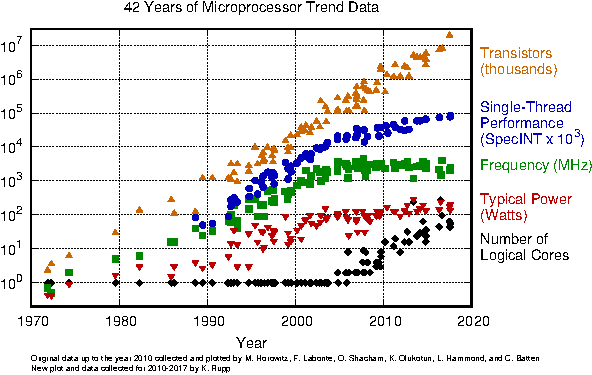
\includegraphics[width=.85\textwidth]{images/42-years-processor-trend.pdf}

		\caption{
			42 years of Multiprocessor Trend Data~\cite{url:microprocessor-trend-data}.
		}\par
		\label{fig.microprocessor-data}
	\end{figure}

% - From multicore to manycores

	However, Figure \ref{fig.microprocessor-data} shows that, in recent years,
	the energy consumption of parallel processors has become as crucial as their
	processing power, which is usually measured by the number of \flops.
	At this point, with the popularization of embedded systems as well as the aim
	to reach the \exascale (10$^{18}$ \flops), a new class of parallel processors,
	named \textit{lightweight} \manycores, emerged to provide high parallelism
	with low-power consumption.

% FROM FUNDAMENTATION
% {
	% With the enhancement of technologies and the reduction of transistors,
	% the number of cores inside a multiprocessor began to scale.
	% Until at some point, these architectures must be called \manycores.
	% However, the line between multi-cores and \manycores is very tenuous.
	% Some researchers stipulate that the difference lies when losing a core
	% does not impact the rest of the system.
	% In this way, \manycores are as multi-cores with tens, hundreds, or even
	% thousands of cores, presenting the most diverse architectural properties.
	% For example, there are \uma/\numa multiprocessors with \simd present on
	% \gpus, and \numa multiprocessors with \mimd as \mppa presented in Section \ref{sec.multiprocessor-hw}.

	% A promising class of \manycores began to emerge, aiming the energy barrier
	% that we will face in the future.
	% \textit{Lightweight Manycores} stand out for their performance compared
	% to their energy consumption.
	% However, due to its particular characteristics, several problems of
	% programmability, portability, and performance are still open.
% }

% - Manycores characteristics
	The \textit{lightweight} \manycores
		(i) integrate thousands of low-power cores in a single die organized in clusters;
		(ii) are designed to cope with \mimd workloads;
		(iii) rely on a high-bandwidth \noc for fast and reliable message-passing communication;
		(iv) present constrained memory systems; and
		(v) frequently feature a heterogeneous configuration.
	Some industry-successful examples of \textit{lightweight} \manycores are
	the \mppa~\cite{DeDinechin2013-1};
	the \epiphany~\cite{olofsson2014}; and
	the \taihulight~\cite{zheng2015}.

% Motivation
% - Difficults from Manycores
	Jointly with further performance scalability and energy efficiency, manycores brought a new
	set of challenges in software development coming from their architectural particularities.
	Precisely, these particularities introduce the following difficulties:
	\begin{itemize}
		\item \textbf{Hybrid programming model:} due to the parallel and distributed nature of
			the architecture, engineers are frequently required to adopt a message-passing
			programming model to deal with the presence of rich \nocs~\cite{kelly2013} that
			interconnects clusters and a shared-memory model inside the cluster.
		\item \textbf{Missing hardware support for cache coherency:} to reduce power consumption,
			theses processors do not feature cache coherency, which in turn forces programmers to
			handle it explicitly in software level and frequently calls out for a redesign in their
			applications~\cite{francesquini2015};
		\item \textbf{Constrained memory system:} the frequent presence of multiple physical
			address spaces and small local memories require data tiling and prefetching to be
			handled by the software~\cite{Castro2016};
		\item \textbf{Heterogeneous configuration:} the different programmable components on
			\textit{lightweight} \manycores turns the actual deployment of applications in a
			complex task~\cite{barbalace2015}.
	\end{itemize}

% - Why is development on manycores difficult?
	Part of these challenges derives from existing \oses and runtimes.
	On the one hand, the complicated portability and scalability of traditional \oses with a
	monolithic kernels, which were designed to homogeneous hardwares, is leading to the development
	of new \oses from scratch~\cite{Baumann2009, kluge2014, nightingale2009, rhoden2011}.
	On the other hand, existing runtimes only partially address some of the programmability issues
	of \textit{lightweight} \manycores, making the process of developing, porting, and maintaining
	applications a challenging task.

% Challenges and Problem Definition
% - How are OSs essential in this context?

% - Why these problems exist? (Because the existing OSes does not handle architecture particularities)
% - These particularities prevent common OSes that easy portated without a complex redesign. And existing OSes does not account some architectural points.

% Goals and Contributions
% - Redesign from scratch around all their tight architectural constraints.
% - Focus on addressing first-order programmability challenges
% - Introducing generic and flexible HAL for lightweight manycores
	% Nexte contexto, o doutorando e coorientador deste trabalho, Pedro H. Penna, mirando a maior programabilidade e portabilidade para lightweight manycores, propoe que sistemas operacionais para essa nova geração de processadores deve ser reprojetada do zero baseando-se em todas as suas restrições arquiteturais.
	% Sua proposta envolve um sistema operacional completo distribuido baseado em uma arquitetura multikernel~\cite{multikernel}.
	% Para isso, baseados em resultados de serviços experimentais desenvolvidos encimado do mppa256~\cite{rmem}, a pesquisa começou buscando resolver os primeiros desafios que surgiram.
	% Especificamente, foi introduzido uma \hal genérica e flexivel para lightweight manycores que lidam com os problemas chaves encontrados no desenvolvimento para esses processadores.
	% Em seguida, a pesquisa seguirá em desenvolver um microkernel para prover os mecanismos básicos para desenvolvimento de um OS completo sobre ele.
	% Por fim, o desenvolvimento de serviços do multikernel serão alcançados.

	We believe that \oses for the next-generation of \textit{lightweight} \manycores must be
	redesigned from scratch to cope with their tight architectural constraints.
	Based on this idea, a new fully-featured distributed \os based on a \multikernel approach~\cite{Baumann2009}
	is being proposed~\cite{penna2017-1,penna2017-2,penna2019}.
	Nanvix features a generic and flexible \hal for \textit{lightweight} \manycores that
	addresses the key issues encountered in the development for these processors.
	On top of the Nanvix \hal, we are simultaneously designing and implementing a \microkernel
	that provides bare bones system abstractions for each cluster.

	In this monograph, we intend to propose a Inter-Cluster Communication Module to the Nanvix \hal
	and port it to the \mppa manycore processor~\cite{DeDinechin2013-1}.
	Using this module, we also pretend design Inter-Cluster Communication Services to the Nanvix \microkernel.
	This work will be done in collaboration with Pedro H. Penna, who is a Ph.D. student at the
	University of Grenoble Alpes, the main developer of Nanvix and the co-advisor of this work.
	Then, we will analyze the performance of the proposed implementation using specific micro-benchmarks.

\section{Objectives}

	This will be written last.
%    Assist to research and develop \hal for \textit{lightweight} manycores.

\subsection{General Objective}

	This will be written last.
%    On the basis of the foregoing, the following general objective and the specific objectives of this project.

\subsection{Specific Objectives}
   \begin{itemize}
		\item This will be written last.
    %    \item Present and discuss hal \textit{lightweight} manycores.
    %    \item Design and develop the Inter-cluster communication module.
    %    \item Assist in the development and improvement of other modules.
    %    \item Perform a performance analysis of the proposed \hal for the \mppa.
   \end{itemize}

\section{Organization Of The Work}

	This will be written last.
\chapter{Background}
\label{ch.fundamentation}

	This chapter presents the background of multiple processor
	systems from a hardware and software perspective.
	Specifically, \autoref{sec.multiprocessors} and \autoref{sec.multicomputers}
	will address details about multiprocessors and multicomputers, respectively.
	Subsequently, \autoref{sec.mppa} will present the \mppa processor.
	Next, \autoref{sec.nanvix} will show an overview of the Nanvix OS.
	So finally, \autoref{sec.inter-cluster-communication} will cover the abstraction
	concepts in the Inter-Cluster Communication Module.

\section{Multiple Processor Systems}
\label{sec.multiple-processor-systems}

	According to Tanenbaum~\cite{tanenbaum:4ed}, there are three models of
	modern multiple processor architectures.
	A shared-memory multiprocessor, a message-passing multicomputer, and a wide
	area distributed systems.
	The sections below address the two first models presenting significant
	hardware and software concepts for the present undergraduate dissertation.

	\subsection{Multiprocessors}
	\label{sec.multiprocessors}

		\begin{figure}[t]
			\centering%
			\caption{Von Neumann Architecture Model.}%
			\label{fig:neumann}%
			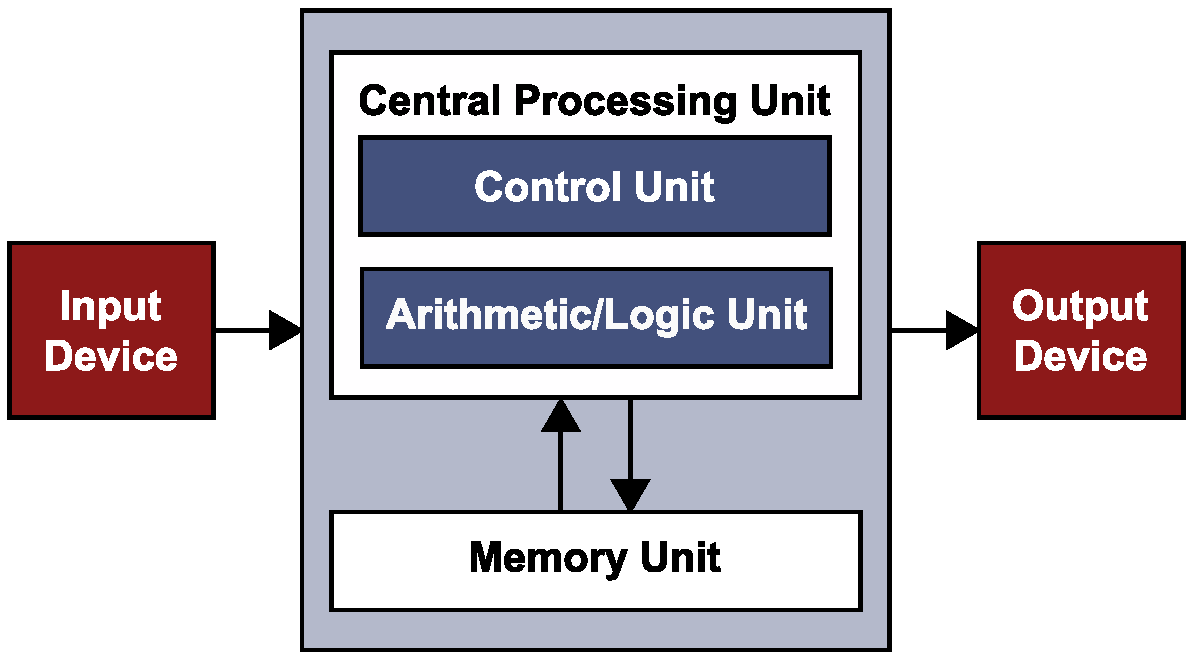
\includegraphics[width=.7\textwidth]{neumann.pdf}%
			\fonte{Adapted from \citeonline{tanenbaum:4ed}.}%
		\end{figure}

		In the early days of electronic digital computing, John Von Neumann
		proposed an architectural model for computers to be easily programmable~\cite{von-neumann:model}.
		As illustrated in \autoref{fig:neumann}, this model describes a \cpu,
		also called core, that loads instructions and data from a \mmu,
		dealing with inputs and generating outputs from/to I/O Devices.
		Modern processors still follow this model, but some components and
		behaviors are specialized or replicated to increase performance.

		In this context, a shared-memory multiprocessor is a computer system
		in which two or more \cpus share full access to a common \ram~\cite{tanenbaum:4ed}.
		Concurrency issues begin to appear where are many \cpus competing for
		shared resources.
		For instance, when many threads of a process competing to read and write a global variable.
		Moreover, some architectures integrate heterogeneous cores introducing portability
		and programmability problems too.
		So, low-level software, such as \os kernels and runtimes, needs to handle those
		issues and provide management systems to user-level.

		\subsubsection{Multiprocessor Hardware}
		\label{sec.multiprocessor-hw}

			The multiprocessors can be usually classified using memory access
			and workflow properties.
			In the first place, the access time to different memory addresses
			split multiprocessors into two groups.
			On the one hand, the group of systems that can read a memory word
			as fast as every other memory word are called \uma multiprocessors.
			On the other hand, \numa multiprocessors do not have this property.

			\begin{figure}[t]
				\centering%
				\caption{Two Bus-Based \uma Multiprocessor Examples.}%
				\label{fig:uma}%

				\subcaptionminipage[fig:uma_a]%
					{.4\linewidth}%
					{Without caching.}%
					{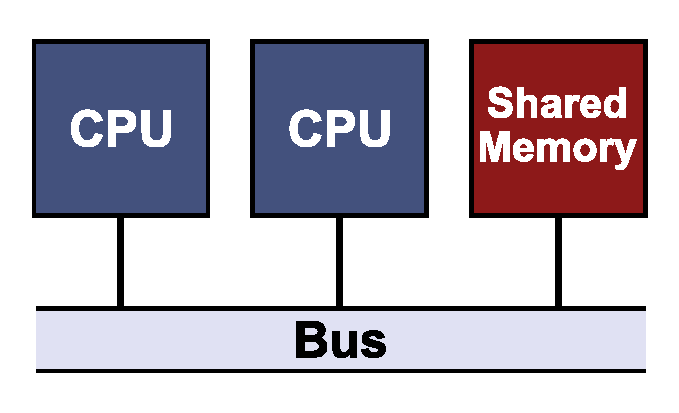
\includegraphics[width=\linewidth]{uma_a.pdf}}%
				\hspace{1.5cm}%
				\subcaptionminipage[fig:uma_b]%
					{.4\linewidth}%
					{With caching.}%
					{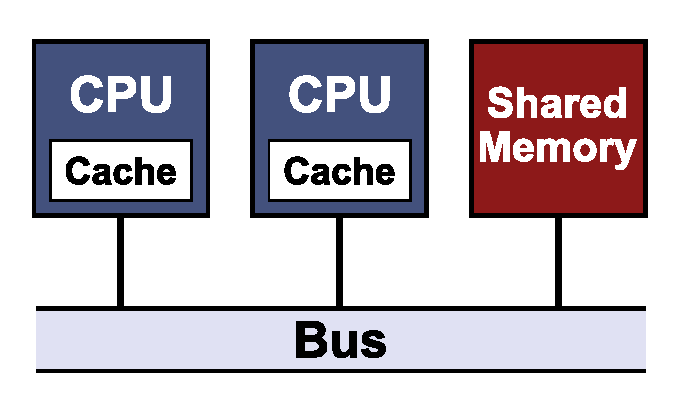
\includegraphics[width=\linewidth]{uma_b.pdf}}%

				\fonte{Adapted from \citeonline{tanenbaum:4ed}.}%
			\end{figure}

			The firsts \uma multiprocessors were bus-based architectures where
			the \cpu wait for the bus channel stays free to perform a memory
			access, as illustrated in \autoref{fig:uma}(a).
			When the number of cores scale, the bus traffic begin to be a
			bottleneck of the system.
			To solve this problem, a small but fast memory level, called cache,
			is added to each \cpu, as depicted in \autoref{fig:uma}(b).
			The cache allowed readings to be resolved locally, reducing traffic
			to the main memory.
			However, many problems of inconsistency and ordering of operations
			on memory arose with the advent of caches.
			For instance, when a write operation dirties a memory address in
			a particular cache, this change must be notified to all other caches.
			Equally important, it is necessary to ensure a specific order in
			the concurrent operations on a given address through different caches.
			The protocols that guarantee these properties are called cache-coherence protocols.

			\begin{figure}[t]
				\centering%
				\caption{\numa Multiprocessor Example.}%
				\label{fig:numa}%
				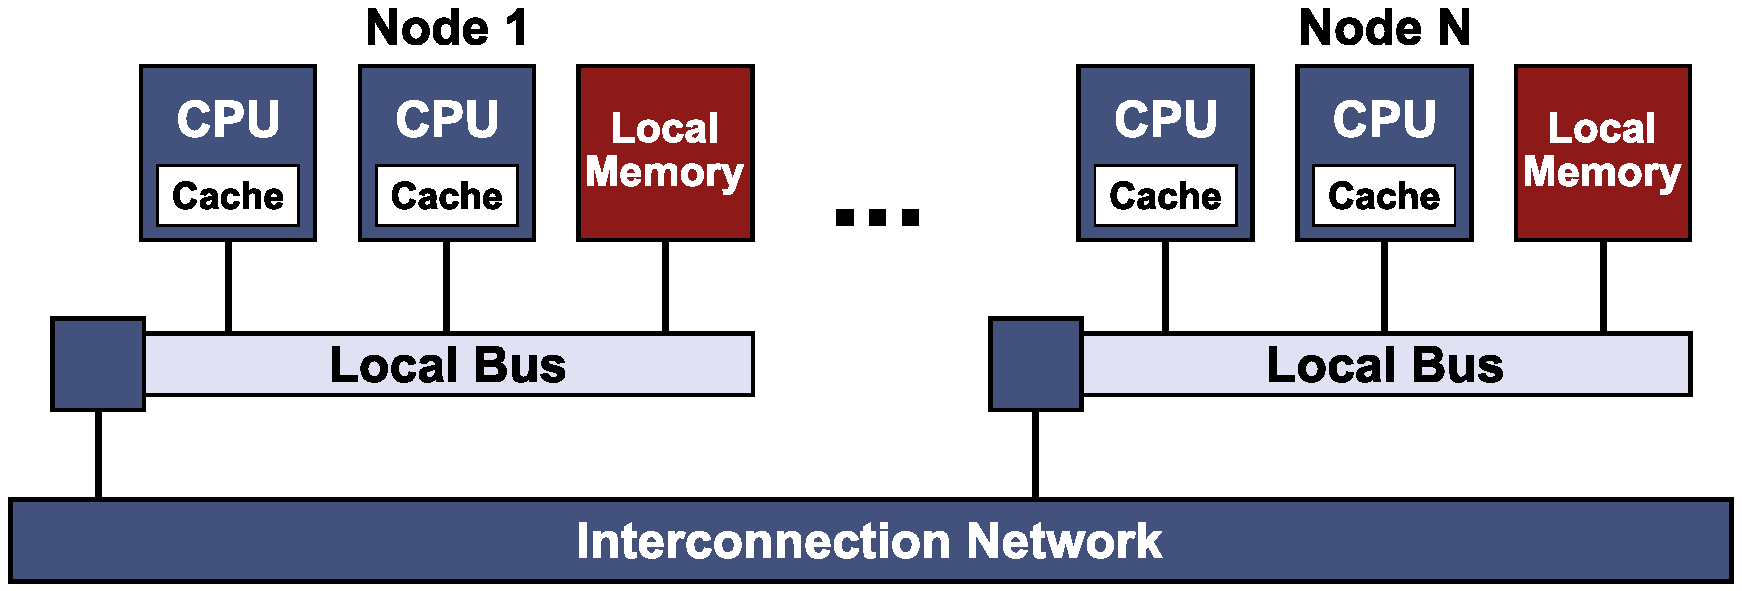
\includegraphics[width=.7\textwidth]{numa.pdf}%
				\fonte{Adapted from \citeonline{tanenbaum:4ed}.}%
			\end{figure}

			Nevertheless, the number of cores in \uma multiprocessors are limited
			to a few dozens of \cpus.
			Thus, to allow hundreds of cores to communicate, \autoref{fig:numa} illustrated
			as that \numa machines provide a single address space visible to all \cpus
			through an interconnection network.
			Therefore, distributing a virtual memory space among local physics memories,
			the access is guaranteed via load and store instructions.
			Although the time to access to remote memory is slower than to local ones,
			this granted that all \uma programs will be able to run on \numa machines
			but with worse performance.

			\begin{figure}[t]
				\centering%
				\caption{Flynn's taxonomy.}%
				\label{fig:flynn}%
				
				\subcaptionminipage[fig:flynn-sisd]%
					{.4\linewidth}%
					{Single Instruction Single Data.}%
					{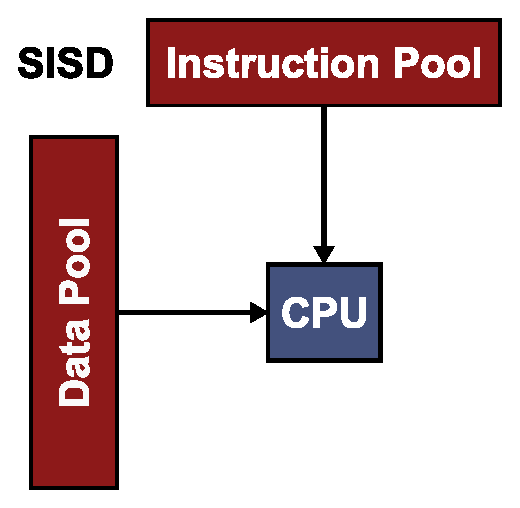
\includegraphics[width=.8\linewidth]{sisd.pdf}}%
				\hspace{1cm}%
				\subcaptionminipage[fig:flynn-simd]%
					{.4\linewidth}%
					{Single Instruction Multiple Data.}%
					{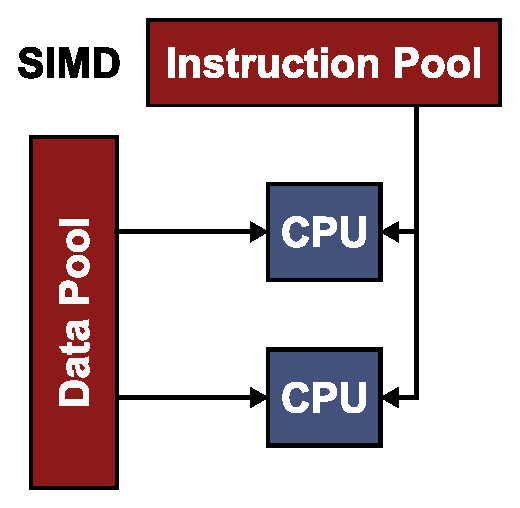
\includegraphics[width=.8\linewidth]{simd.pdf}}%

				\subcaptionminipage[fig:flynn-misd]%
					{.4\linewidth}%
					{Multiple Instruction Single Data.}%
					{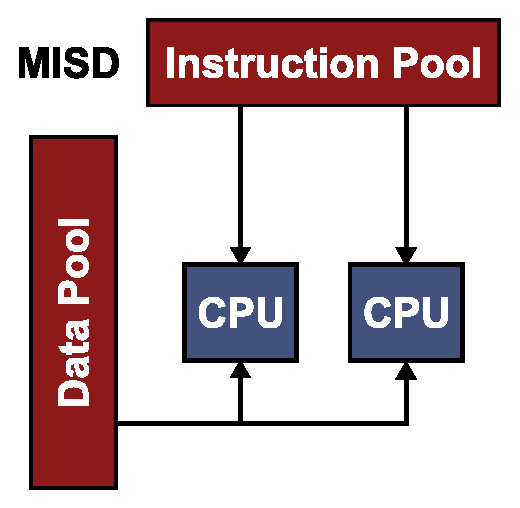
\includegraphics[width=.8\linewidth]{misd.pdf}}%
				\hspace{1cm}%
				\subcaptionminipage[fig:flynn-mimd]%
					{.4\linewidth}%
					{Multiple Instruction Multiple Data.}%
					{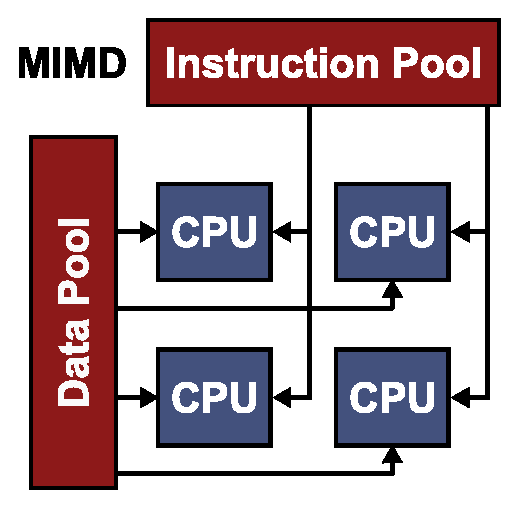
\includegraphics[width=.8\linewidth]{mimd.pdf}}%

				\fonte{Adapted from \citeonline{url:flynn}.}%
			\end{figure}

			In the second place, the workflow classification proposed by Michael J. Flynn~\cite{flynn:1972},
			split multiprocessors architecture based on the number of concurrent
			instruction and data streams available, as depicted in \autoref{fig:flynn}.
			First, the most straightforward class, \sisd describes a sequential
			machine which exploits no parallelism in either the instruction or
			data streams, like older uniprocessor machines.
			Second, \simd uses multiple functional units to replicate and operate
			a single instruction over multiples different data streams, like \gpu.
			Third, the most uncommon class, \misd describe multiprocessors that
			apply multiple instructions streams over one data stream.
			Systems that need fault tolerance uses theses multiprocessors, like
			modern flight control systems.
			Finally, a \mimd architecture has multiple processors simultaneously
			executing different instruction on different data, like \xeonphi.

			Currently, two categories of multiprocessors attract attention, the \cmp and \mpsoc.
			\cmps are multicore commercials, which follow a symmetric architecture,
			integrating two or more identical cores into a single die.
			They can have private or shared cache levels, and always share access
			to the RAM.
			Alternatively, \mpsocs are designed with an asymmetric architecture,
			have in addition to the main cores, specialized \cpus in particular
			functions, \eg audio and video encoders, encryption, becoming truly
			complete computer systems on a single chip.
			All these cores are linked to each other by an on-chip network-based
			communications subsystem, called \noc.
			The \noc improve scalability and power consumption compared to other
			communication subsystem designs.

		\subsubsection{Multiprocessor \oss}
		\label{sec.multiprocessor-os}

			\oss are a fundamental part of any computer system.
			They act as an intermediary between users and hardware, with the
			purpose to provide an environment in which users can run programs
			in a conveniently and efficiently manner~\cite{Silberschatz:9ed}.
			Many \os approaches exist in multiprocessor systems.
			In particular, three of them express accurately the difficulties
			of developing \oss targeting the concurrency issues existing in
			such systems.
			Those models are called Replicated, Master-Slave, and Symmetric \os.

			\begin{figure}[t]
				\centering%
				\caption{Replicated \os Model.}%
				\label{fig:replicated-os}%
				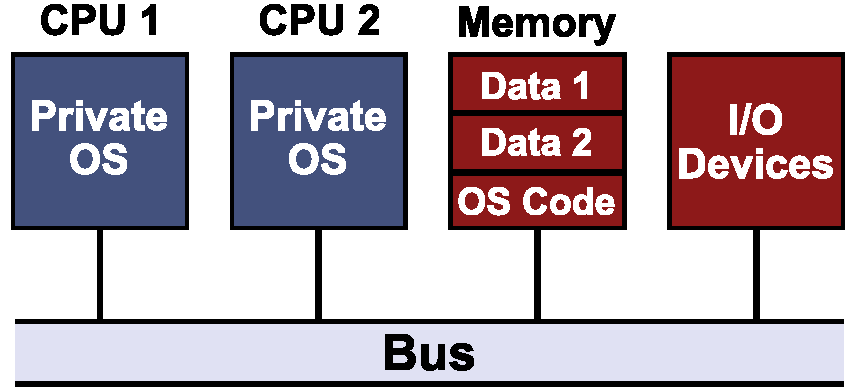
\includegraphics[width=.55\textwidth]{replicated-os.pdf}%
				\fonte{Adapted from \citeonline{tanenbaum:4ed}.}%
			\end{figure}

			The Replicated Model is the simplest way to develop an \os for a
			parallel architecture.
			It only needs to replicate all the internal \os structures for each core.
			\autoref{fig:replicated-os} shows how this model allocates fixed memory spaces
			between the cores, giving each of them its private \os.
			The system calls are performed by the calling \cpu, avoiding concurrency issues.
			Also, a producer-consumer model is sufficient for two different \cpus to communicate.

			However, this model has imperceptible aspects~\cite{tanenbaum:4ed}.
			First, since each \cpu has its own process and page tables, it is impossible
			to optimize the use of resources.
			For instance, if many of processes are waiting for use an overloaded \cpu,
			it is impossible to migrate them to an available \cpu.
			Second, operations with I/O devices can introduce inconsistency problems
			such as the same disk block operated by different \cpus.
			Finally, replication of the internal \os structures makes this model
			impractical for systems with memory constraints.

			\begin{figure}[t]
				\centering%
				\caption{Master-Slave \os Model.}%
				\label{fig:master-slave-os}%
				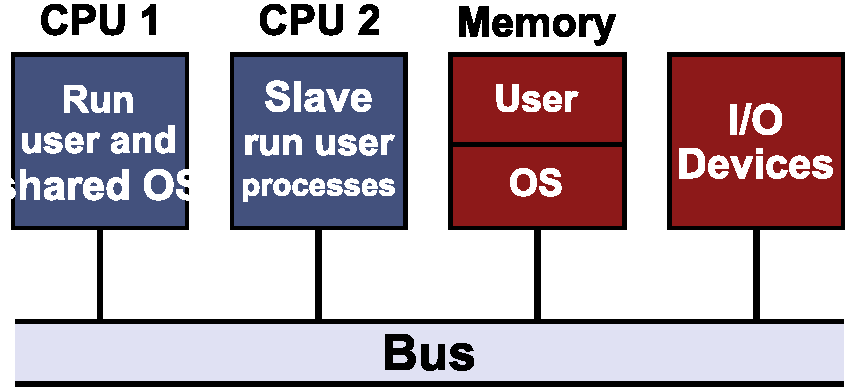
\includegraphics[width=.55\textwidth]{master-slave-os.pdf}%
				\fonte{Adapted from \citeonline{tanenbaum:4ed}.}%
			\end{figure}

			The Master-Slave model began to attract attention with the return of
			processors with no cache coherence.
			As \autoref{fig:master-slave-os} shows, there is only one copy of
			the internal \os structures, and they all belong to a single \cpu, called master.
			In this way, all system calls performed by a worker \cpu, called slave,
			are redirected to the master.
			With these changes, this model solves the problems of the previous model
			by using only one copy of the data structures.
			For illustration, processes and memory pages can be scheduled and
			distributed dynamically to any \cpus.
			However, when adopting a centralized approach, the master can become
			the bottleneck of the system if it can not handle the number of the
			incoming requisition.

			\begin{figure}[t]
				\centering%
				\caption{Symmetric \os Model.}%
				\label{fig:smp-os}%
				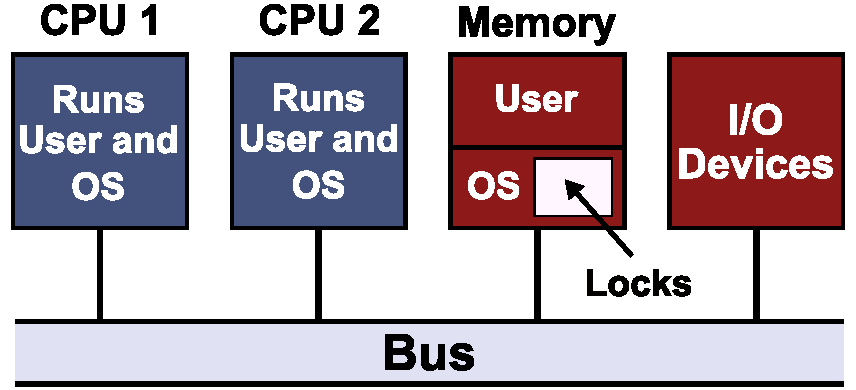
\includegraphics[width=.55\textwidth]{symmetric-os.pdf}%
				\fonte{Adapted from \citeonline{tanenbaum:4ed}.}%
			\end{figure}

			Finally, the Symmetric model, called \smp, eliminates the centralization
			problem of the foregoing model, as illustrated in \autoref{fig:smp-os}.
			So, there is still only one copy of the \os structures but shared in memory.
			When a \cpu makes a system call, it loads the structures and operates on them.
			Consequently, processes and memory pages also continue to be dynamically balanced.
			The difficulties introduced by this model lie in concurrency for \os structures.
			Depending on how the critical regions are managed, the performance of the system
			may be equivalent to the Master-Slave model. So the hardest part is breaking the
			\os into critical regions that will run on different \cpus, where one core does
			not affect the execution of another or fall into a deadlock~\cite{tanenbaum:4ed}.
			Besides, if the hardware does not support cache coherence, the process of
			invalidating the cache may also introduce serious performance problems in \oss of this type.

			As it can be noted, the software is always lagging behind the constant hardware advances.
			Many solutions may work very well in specific contexts but should be chosen with care.
			In some cases, in order to extract the maximum performance from a system, it will be
			necessary to redesign the whole process from scratch.

	\subsection{Multicomputers}
	\label{sec.multicomputers}

		Increasing the number of cores and still providing a shared memory in a
		single die is very expensive and challenging.
		However, it is more simple and cheap to interconnect more straightforward
		computers in a high-speed network. The result is a clustered archietcture.
		Despite the problem of developing networks and high-speed interfaces
		for communication of the nodes, it is analogous to the problem of
		providing a shared memory in multiprocessors.
		Nevertheless, the expected communication times will be in the
		microseconds, as opposed to nanoseconds of the multiprocessors,
		making things simpler~\cite{tanenbaum:4ed}.

			\subsubsection{Multicomputer Hardware}
			\label{sec.multicomputers-hw}

				A multicomputer node can be considered as an elementary computer, with one or
				more multiprocessors, local \ram and I/O devices.
				In many cases, there is no need for monitors or keyboards, only the
				network interface.
				In this way, it is possible to integrate hundreds or even thousands
				of nodes providing the vision of a single computer.

				\begin{figure}[t]
					\centering%
					\caption{Network Topologies Examples.}%
					\label{fig:net-topologies}%

					\subcaptionminipage[fig:net-start]%
						{.25\linewidth}%
						{Star.}%
						{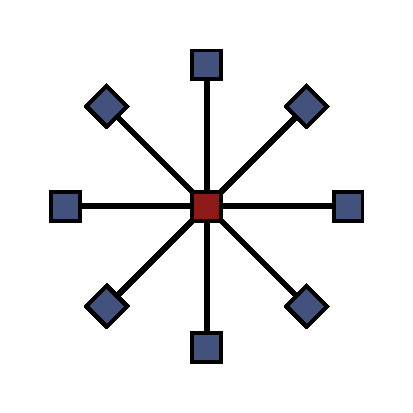
\includegraphics[width=\linewidth]{net-star.pdf}}%
					\hspace{1cm}%
					\subcaptionminipage[fig:net-ring]%
						{.25\linewidth}%
						{Ring.}%
						{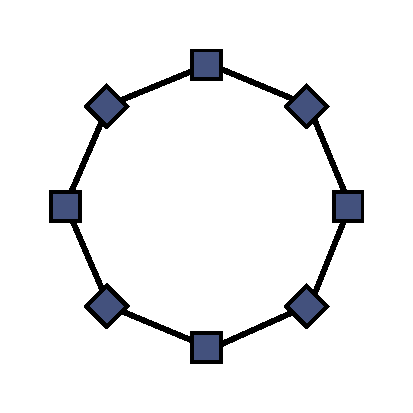
\includegraphics[width=\linewidth]{net-ring.pdf}}%
					\hspace{1cm}%
					\subcaptionminipage[fig:net-grid]%
						{.25\linewidth}%
						{Grid.}%
						{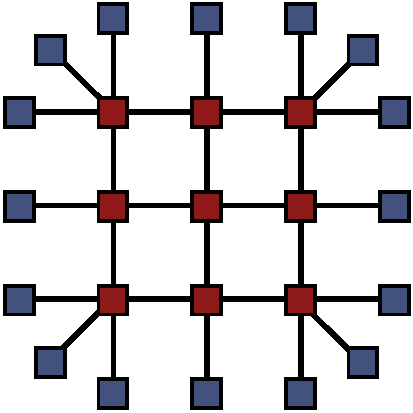
\includegraphics[width=\linewidth]{net-grid.pdf}}%

					\subcaptionminipage[fig:net-torus]%
						{.25\linewidth}%
						{Torus.}%
						{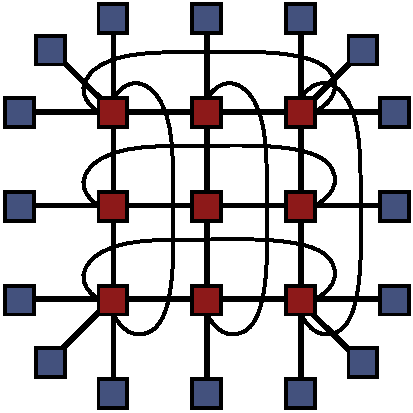
\includegraphics[width=\linewidth]{net-torus.pdf}}%
					\hspace{1cm}%
					\subcaptionminipage[fig:net.grid-3d]%
						{.25\linewidth}%
						{Grid 3D.}%
						{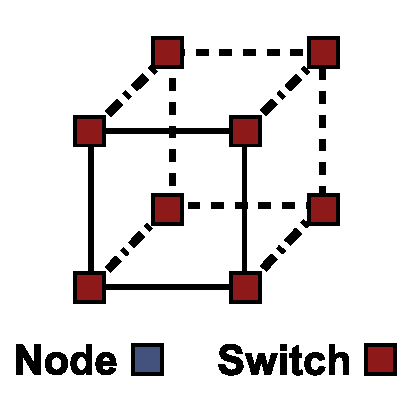
\includegraphics[width=\linewidth]{net-3d.pdf}}%

					\fonte{Adapted from \citeonline{tanenbaum:4ed}.}%
				\end{figure}

				A switch set is organized into different topologies to interconnect
				the nodes of a multicomputer.
				As illustrated in \autoref{fig:net-topologies}, there are a
				variety of topologies with their own characteristics.
				For instance, commercial multicomputer usually uses bi-dimensional
				topologies such as \textit{grid} or \textit{mesh} because they present
				regular behavior and can scale easily.
				When the goal is to provide higher fault tolerance, in addition to the
				smaller path between two points, the \textit{torus} variant implement
				connections between the extreme points of the \textit{grid}.
				Even multi-dimensional topologies can be used, all depending on the
				characteristics expected from the network.

				There are two types of switching schemes in the multicomputer network.
				The \textit{store-and-forward packet} switching scheme breaks the message
				into fixed-size packets.
				The packets are copied and moved between the switches following a
				routing algorithm until they reach the destination.
				Although flexible and efficient, this scenario can generate a variable
				latency in packet delivery.
				The other scheme, called \textit{circuit switching}, performs a resource
				allocation protocol through all path from source to the destination.
				This protocol ensures a steady communication stream, although the
				slow start and possible sub-utilization of the resources.

			\subsubsection{Low-Level Communication Software}
			\label{sec.multicomputers-low-sw}

				\begin{figure}[t]
					\centering%
					\caption{Simple Multicomputer Example.}%
					\label{fig:multicomputer}%
					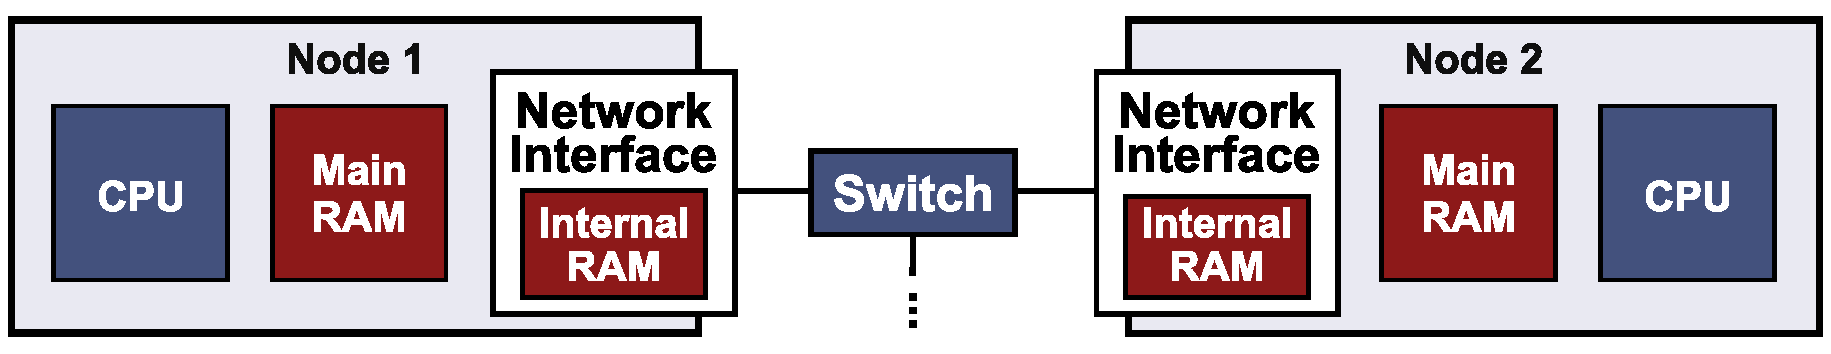
\includegraphics[width=.8\textwidth]{multicomputer.pdf}%
					\fonte{Adapted from \citeonline{tanenbaum:4ed}.}%
				\end{figure}

				Multicomputer nodes are interconnected to each other through network interfaces.
				Because these boards are built and connected to \cpus and \ram,
				they have substantial impacts on system performance and \os design.
				Virtually, interfaces have enough \ram space to receive/send packets.
				If this address space is actually in main memory, we fall into the same
				problem of multiprocessors in the struggle for the use of the bus channel.
				Thus, in general, network cards have a dedicated memory so as not to
				generate bottlenecks in access to main memory, as illustrated in \autoref{fig:multicomputer}.

				However, excessive packet copying can degrade the performance of the system.
				In an ideal scenario, four end-to-end copies would be needed:
				(i) from the \ram of the sender to the interface memory;
				(ii) from the interface to the network;
				(iii) from the network to the memory of the target interface, and, finally,
				(iv) to the \ram of the recipient.
				However, the number of copies may increase further, depending on how the \os
				implements communication services on available hardware.
				For instance, mapping the interface into the kernel address space
				rather than the user-space, an extra copy to an internal kernel
				buffer is required.
				Thus, for performance reasons, modern systems already map the interfaces
				to user-space address.
				Nonetheless, they introduce problems of concurrency between the various
				users by the communication resources.

				Processors may also have one or more \cpus specialized in
				communication procedures, called \dma.
				\dmas can make copies between system memories, send/receive packets
				without the main \cpus intervention. This reduces considerably wasted cycles due to 
				network interfaces communication and/or main memory access bottlenecks.
				However, such intermediate copies lead to overhead on system structures,
				such as cache, \tlb, or page management.
				Furthermore, this introduces concurrency issues in the interaction between
				\cpus and existing \dma channels.

			\subsubsection{User-Level Communication Software}
			\label{sec.multicomputers-user-sw}

				The low-level mechanisms discussed above allow \cpus on different
				computers to communicate through the messages exchange by
				send/receive primitives.
				The basic configuration needed for send primitive is knowing the
				recipient identifier and the message.
				Moreover, the receive primitive needs to identify which of
				the network interfaces it should configure and where to write the
				incoming data.

				\begin{figure}[t]
					\centering%
					\caption{Calls Types.}%
					\label{fig:calls-types}%

					\subcaptionminipage[fig:call-sync]%
						{.9\linewidth}%
						{Synchronous Call on Sender Node.}%
						{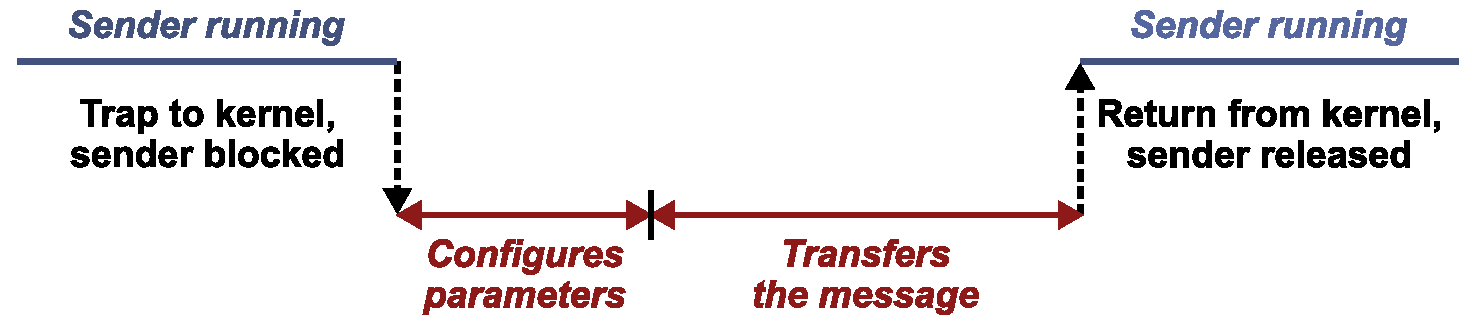
\includegraphics[width=\linewidth]{call-sync.pdf}}%

					\hfill

					\subcaptionminipage[fig:call-async]%
						{.9\linewidth}%
						{Asynchronous Call on Sender Node.}%
						{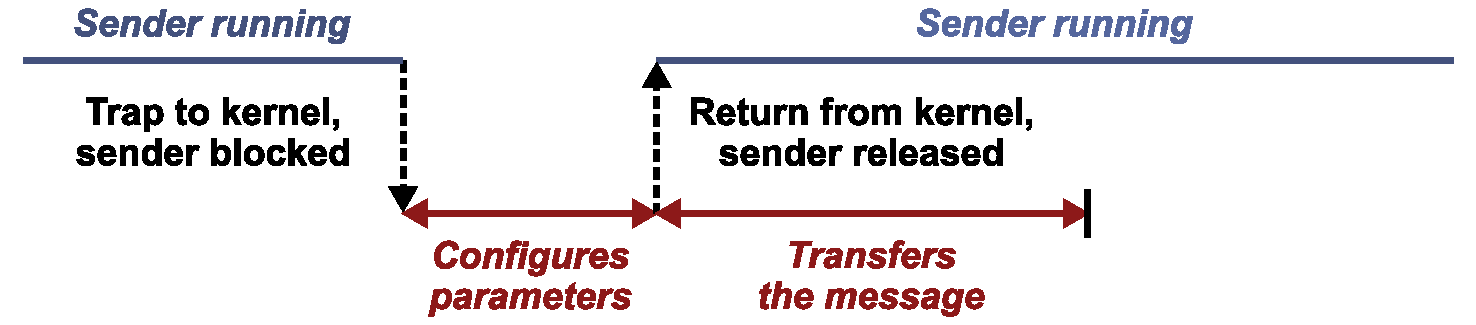
\includegraphics[width=\linewidth]{call-async.pdf}}%

					\fonte{Adapted from \citeonline{tanenbaum:4ed}.}%
				\end{figure}

				\autoref{fig:calls-types} illustrates the two approaches to implement
				these primitives, either through blocking or non-blocking calls.
				Blocking calls, called \textit{synchronous calls}, block the requesting \cpu
				until complete the procedure.
				Non-blocking calls, called \textit{asynchronous calls}, return control to the
				\cpu while the procedure is still in progress.
				Although asynchronous calls provide better performance than
				synchronous ones, they introduce some disadvantages where the sender/receiver
				cannot use the message buffer before the operation is complete.
				According to Tanenbaum~\cite{tanenbaum:4ed}, there are four ways to implement
				a send primitive:
				\begin{itemize}
					\item \textit{Blocking sending:} \cpu hibernates or schedules another
						process, while the message is transmitted;
					\item \textit{Non-blocking sending with copying:} realizes an extra copy of
						the message to a kernel buffer, degrading performance;
					\item \textit{Non-blocking sending with interrupt:} notifies the \cpu
						when the send finishes, where the buffer must remain untouchable,
						difficulting the programmability;
					\item \textit{\cow:} management of buffers to make an extra copy only
						when needed, but can copy unnecessarily.
				\end{itemize}

				Analogously, there are other four forms to implement a receive primitive:
				\begin{itemize}
					\item \textit{Blocking receive:} \cpu hibernates or schedules another
						process until a message is received;
					\item \textit{Non-Blocking receive with messages pool:} \cpu creates
						a buffer to store incoming messages, then consumes from it when
						there is some message available, requiring synchronization;
					\item \textit{Non-Blocking receive with Pop-up Threads:} creates a specific
						thread upon receiving a message to perform the necessary operations,
						but consumes resource for creating and destroying the thread;
					\item \textit{Non-Blocking receive with interrupt handlers:} the receiver
						is interrupted to execute a handler when receiving a message, resulting
						in a better performance than creating a thread but difficults
						the programmability.
				\end{itemize}

				Some of the implementation approaches may be hardware dependent.
				However, choosing the ideal approach is still the responsibility of the \os designer.
				Even so, the distributed nature of multicomputers forces developers to
				use a messaging strategy regardless of what the hardware has to offer.

\section{The MPPA-256 Lightweight Manycore Processor}
\label{sec.mppa}

	\begin{figure}[t]
		\centering%
		\caption{Architectural overview of the \mppa processor.}%
		\label{fig:mppa-arch}%
		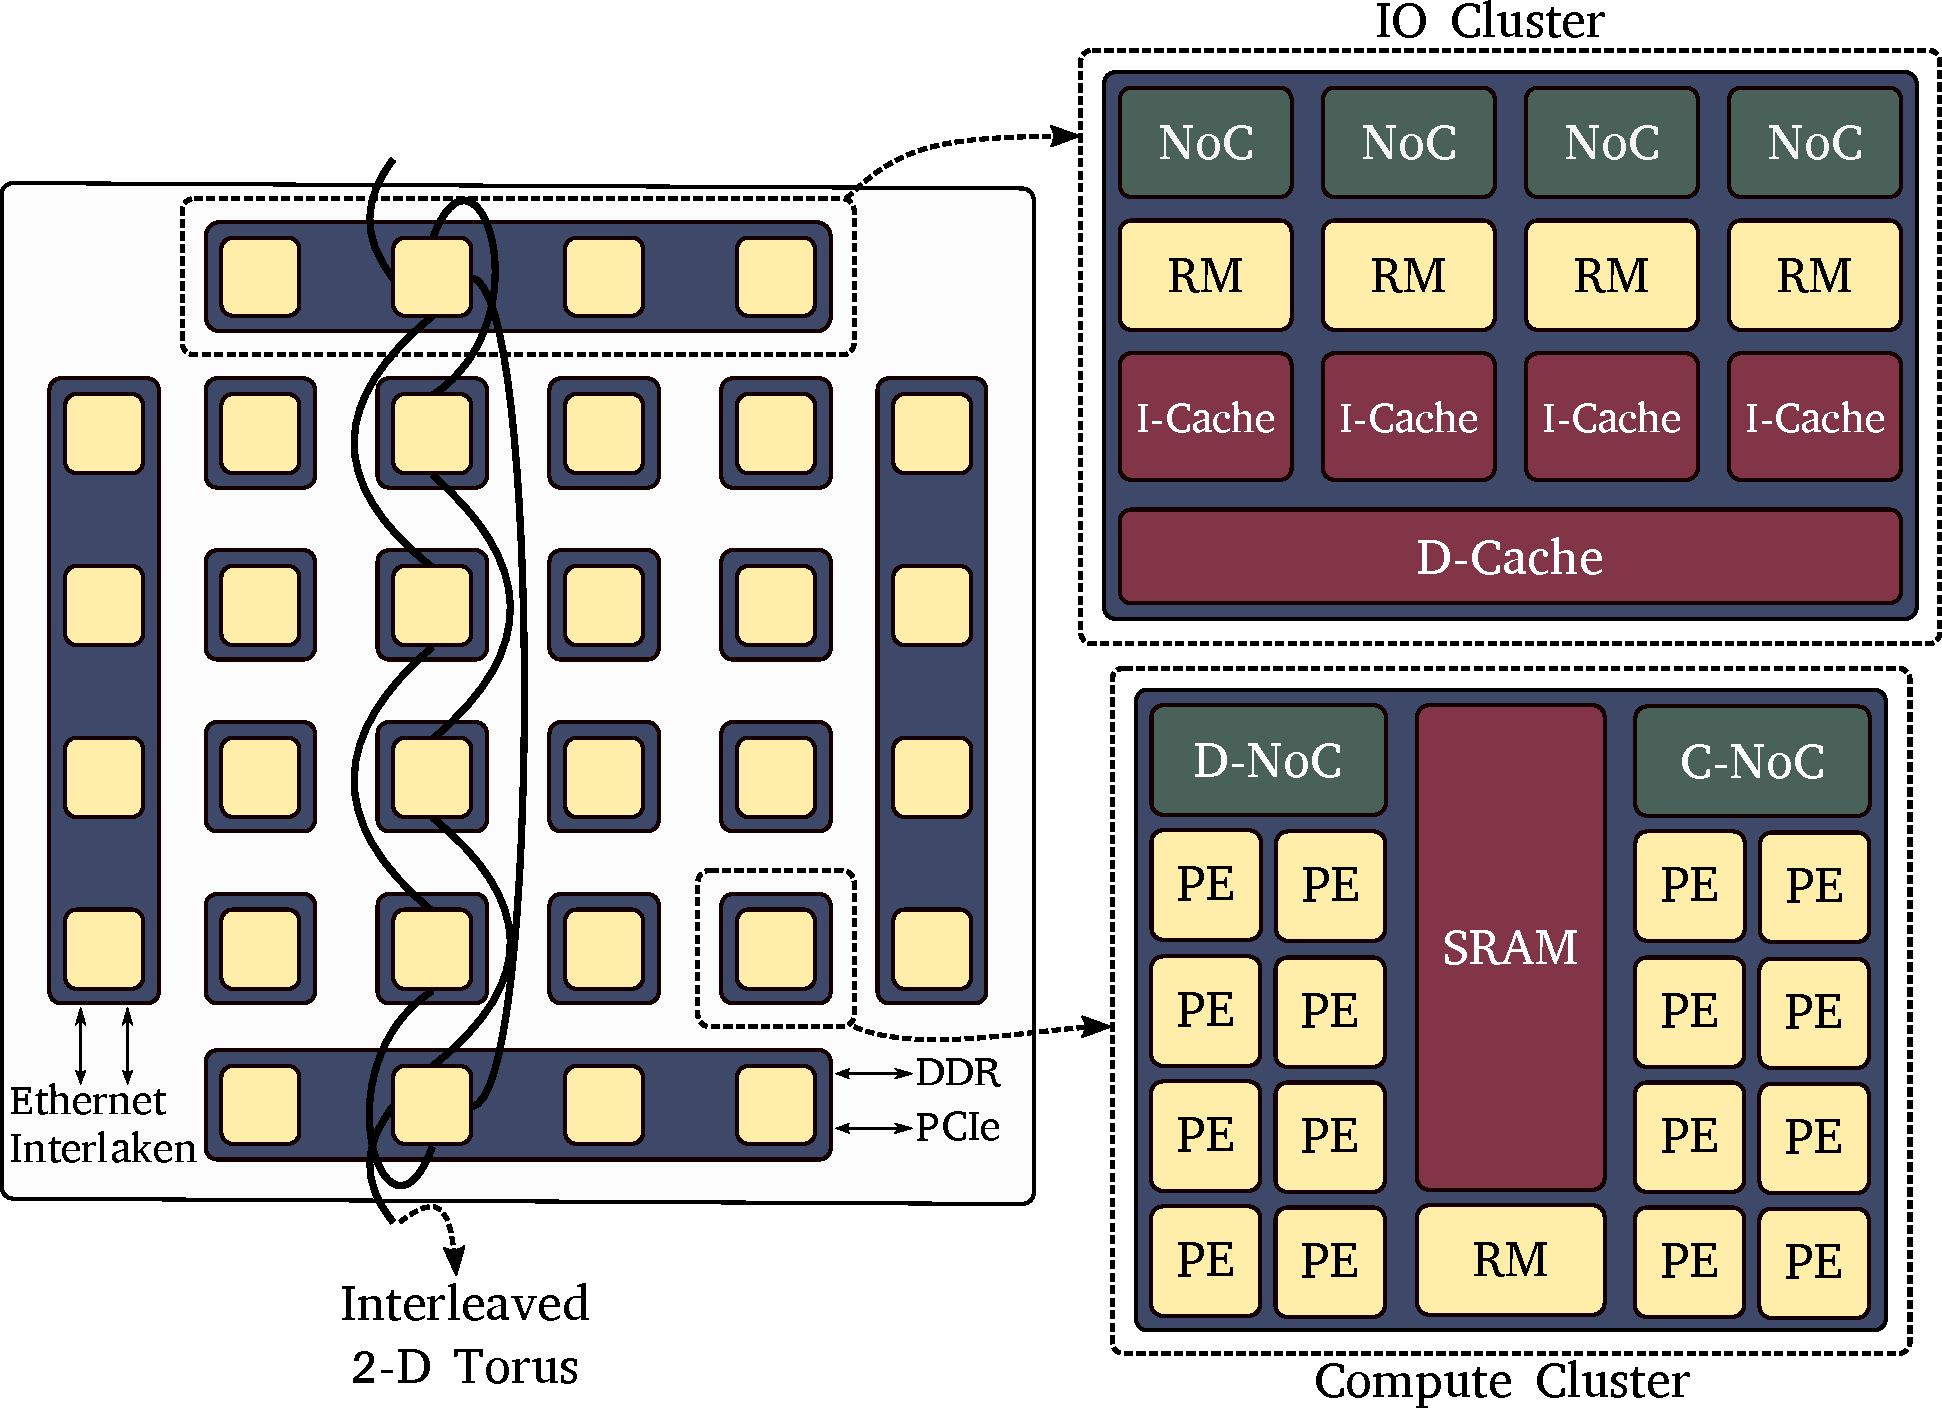
\includegraphics[width=.7\textwidth]{arch-mppa.pdf}%
		\fonte{\citeonline{Penna2018}.}%
	\end{figure}

	The \mppa is a high-performance, lightweight multicore processor
	developed by the French company Kalray.
	Developed to handle \mimd workloads, \mppa mixes features of
	multiprocessors and multicomputers on a single chip.
	Precisely, the multiprocessor model is used inside a cluster
	to coordinate the cores and the local resource balancing, and
	follows a multicomputer model in inter-cluster communication.

	As illustrated by \autoref{fig:mppa-arch}, the used version of
	the architecture, called Bostan, has 256 general-purpose cores and
	32 firmware cores, called \pes and \rms, respectively.
	The processor use 28~mm CMOS technology and all cores run at 500~MHz.
	Besides, all cores have caches and \mmus with software-managed \tlbs.
	Finally, the 288 cores are grouped into 16 \cclusters, dedicated to
	the payload, and 4 \ioclusters, responsible for communicating with peripherals.

	Each \ccluster features 16 \pes, an \rm, an \noc interface and 2~MB of \sram.
	The hardware does not support cache coherence to improve energy consumption.
	On the other hand, \ioclusters have only 4 \rms with cache coherence support,
	4 \noc interfaces, and 4~MB of local \sram added to 4~GB of \dram.
	The address space on each cluster is private, forcing exchange messages
	by one of two different interleaved 2-D Torus \nocs.
	On the one hand, the \cnoc is exclusive to 64-bit control messages,
	usually used for synchronization.
	On the other hand, intense exchange data occurs through the \dnoc.
	Additionally, all clusters have available \dmas associated with each
	\noc interfaces to handle communication issues.

	As discussed in \autoref{sec.multicomputers-user-sw}, the \noc interfaces
	expose communication resource to perform send and receive primitives
	like network interfaces.
	Accurately, they summarize the following resources:

	\begin{itemize}
		\item 128 slots for receiving commands;
		\item 256 slots for receiving data;
		\item 4 channels for sending commands;
		\item 8 channels for sending data, and;
		\item 8 $\mu$threads for sending asynchronous data (each of which must
			to be associated with a transfer channel).
	\end{itemize}

	The configuration of these features is accomplished by a mix between
	writing on \dma registers and performing syscalls to a hypervisor
	that virtualizes the \mppa hardware.

\section{Nanvix: An Operating System for Lightweight Manycores}
\label{sec.nanvix}

	Current research efforts on Nanvix \os focus on the programmability and portability
	challenges that have arisen with \textit{lightweight \manycores}~\cite{christgau2017, gamell2012, serres2011}.
	We believe that significant barriers will still arise in this scenario, and the
	solution is to rethink \os design from scratch~\cite{penna:compas19, penna2019}. 
	In this context, the Nanvix \os aims improving programmability and
	software portability in lightweight manycores by means of a fully-featured
	\posix-compliant \os~\cite{penna:compas19}.
	It follows a multi-kernel design where OS services are scattered across cores and
	interacting with user processes through a Client-Server approach.
	
	Nanvix \os can be divided into three distinct kernels, \multikernel,
	\microkernel, and \hal.
	The \multikernel is made up of high-level OS services, \eg shared memory
	regions and name resolution.
	It exports both the client and server interfaces, both developed above
	the \microkernel services.
	On top of the \hal, The \microkernel follows the Master-Slave \os model
	to avoid the problem of the lack of coherence of many manycores.
	It shall run in each cluster and provide bare bones system abstractions,
	such as thread management, thread synchronization,
	virtual memory support and communication services.
	And finally, the next section will introduce \hal.

	\subsection{Hardware Abstract Layer (HAL)}
	\label{sec.hal}

		Nanvix \os proposes a generic and flexible \hal around the
		intrinsic architectural characteristics of the \textit{lightweight \manycores}.
		In this undergraduate dissertation, we  focus on the development of \hal
		to \mppa~\cite{DeDinechin2013-1}.
		However, other efforts have also been done for other platforms such
		as~\optimsoc~\cite{Wallentowitz2013}.

		Unlike other approaches that aim to design a fully-featured \os~\cite{Baumann2009,kluge2014,nightingale2009,rhoden2011},
		the \hal belongs to one level below.
		It is the first layer on top of the hardware and should provide a standard
		view of these emerging processors for a client applications, \eg \os.
		As illustrated in \autoref{fig:hal-struct}, this \hal is structured in
		two major logic layers: \textit{Cluster Abstraction Layer} and \textit{Processor Abstraction Layer}.

		\begin{figure}[t]
			\centering%
			\caption{Structural overview of the proposed \hal.}%
			\label{fig:hal-struct}%
			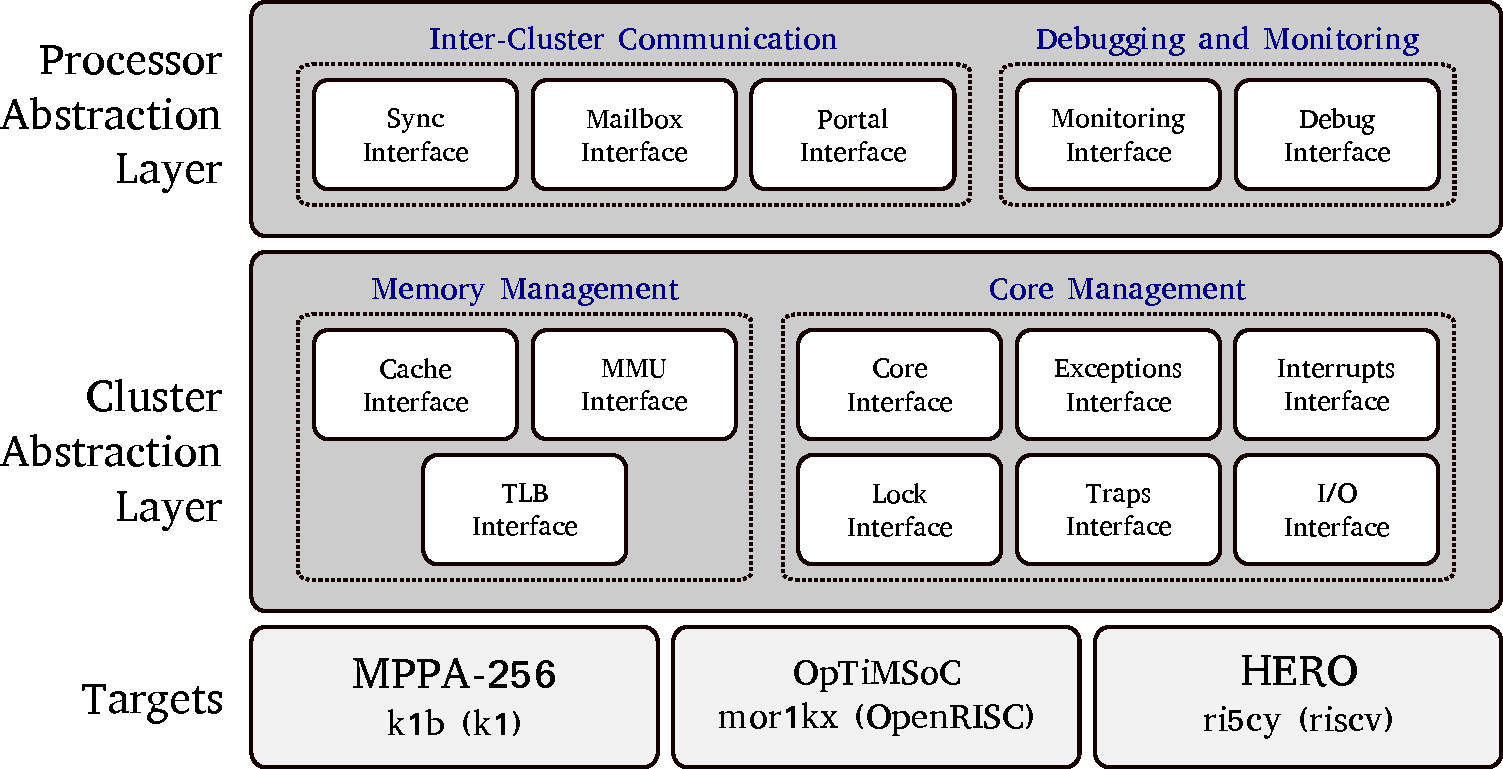
\includegraphics[width=.8\textwidth]{hal-struct.pdf}%
			\fonte{\citeonline{penna:compas19}.}%
		\end{figure}

		The \textit{Cluster Abstraction Layer} encapsulates the management of a single cluster.
		It provides two modules, \textit{Core Management}, and \textit{Memory Management}.
		The \textit{Core Management Module} aims to provide to a client application a complete
		thread synchronization and management system, rich support of handling
		interrupts/exceptions, and an adequate system call interface.
		The \textit{Memory Management Module} provides a uniform view of the \tlbs
		and paging systems with maintenance routines for them and the cache.
		Therefore, some design decisions are made to create interfaces that are not
		dependent on the underlying hardware.
		For example, a context switch mechanism was not provided in the
		Core Management module because this would force the client \os
		to write code in assembly, hurting the conceptual idea of the \hal.

		The \textit{Processor Abstraction Layer}, in particular, embraces
		architectural features related to multiple clusters.
		The \textit{Inter-Cluster Communication Module}, the focus of
		this undergraduate dissertation, exports three main abstractions to allow the
		cluster to exchange data between them, based on ideas proposed along with the
		\nodeos distributed runtime system~\cite{DeDinechin2013-1}.
		Lastly, the \textit{Monitoring and Debugging Module}, as the
		name shows, exports routines to aid debugging and extraction
		of diagnostics about hardware metrics, such as the number of
		page-fault or detour taken.

		\subsubsection{Inter-Cluster Communication Module}
		\label{sec.inter-cluster-communication}

			The following sections conceptually present the three abstractions
			exported by \hal and which will be implemented on the \mppa.
			They are the \sync, \mailbox, and \portal abstraction.
			The purpose of developing more specific abstractions than
			send and receive primitives, described in \autoref{sec.multicomputers-user-sw},
			is to provide more precise and easy-to-use mechanisms for
			\os and client applications.
			On top of them, it is possible to create all kinds of essential
			services such as message passing and synchronization,
			to more elaborate services such as shared memory regions~\cite{penna:rmen}.

			A related point to consider is that mechanisms described below refer
			to interactions between distinct clusters only.
			As described in \autoref{sec.multicomputers-user-sw}, these system
			abstractions can use the communication primitives, \ie send and receive
			primitives, to export more elaborate services.
			The behavior expected can be simulated both through synchronous calls
			and asynchronous calls, depending only on hardware support.
			In the same way, it is worth be noted that the small messaging exchange
			is decoupled from abstraction to intense data transfer.
			The motivation for this, as other details, is to exhibit better control
			over the \qos to the higher layers.
			For instance, the use of distinct \nocs for each service.

			\subsubsubsection*{Sync Abstraction}
			\label{sec.sync-abs}

				\begin{figure}[t]
					\centering%
					\caption{Synchronization Abstraction Concept.}%
					\label{fig:conpt_sync}%

					\subcaptionminipage[fig:conpt_sync-create]%
						{.7\linewidth}%
						{N Slaves notify the Master.}%
						{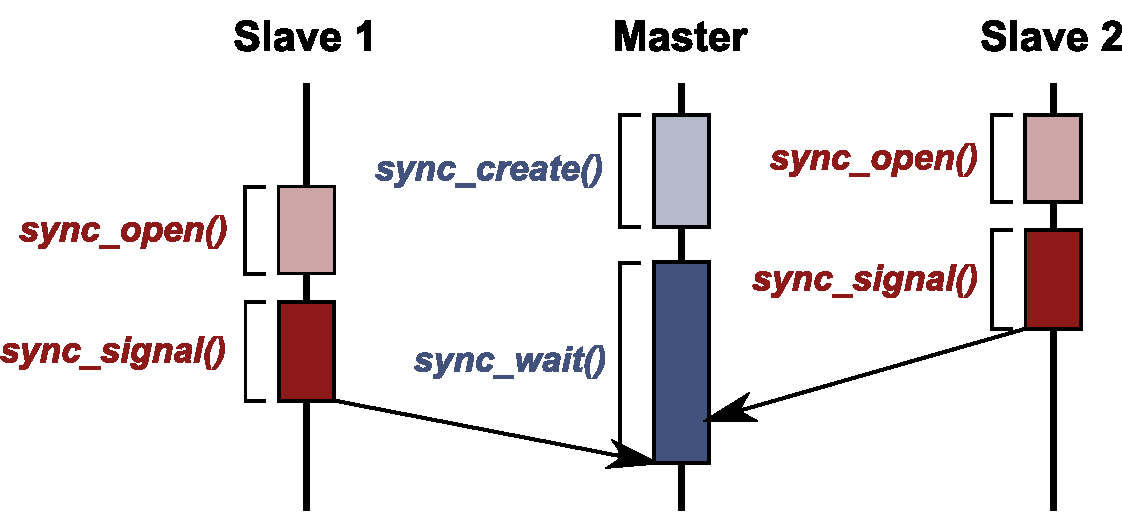
\includegraphics[width=\linewidth]{sync-create.pdf}}%

					\hfill

					\subcaptionminipage[fig:conpt_sync-open]%
						{.7\linewidth}%
						{The Master notify N Slaves.}%
						{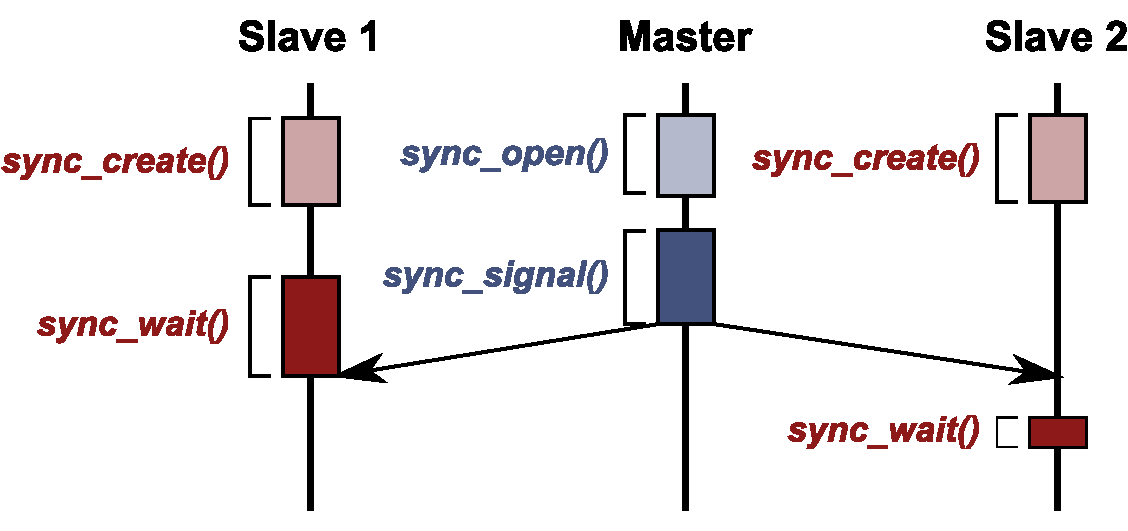
\includegraphics[width=\linewidth]{sync-open.pdf}}%

					\fonte{Developed by the Author.}%
				\end{figure}

				The \textit{Synchronization Abstraction}, called \sync, proves bare bones
				for cluster synchronization.
				From this, it is possible to create distributed barriers.
				For instance, a set of clusters can wait for a notification coming
				from a specific cluster.
				The behavior is analogous to the \posix signal abstraction, but the \sync
				provides only the case of notification.
				Specifically, as can be seen in \autoref{fig:conpt_sync}, the
				cardinality of the operation is N:1, where N clusters wait for 1 Cluster
				to send a notification.

			\subsubsubsection*{Mailbox Abstraction}
			\label{sec.mailbox-abs}

				\begin{figure}[t]
					\centering%
					\caption{Mailbox Abstraction Concept.}%
					\label{fig:conpt_mailbox}%

					\subcaptionminipage[fig:conpt_mailbox-logical]%
						{.5\linewidth}%
						{Conceptual Overview.}%
						{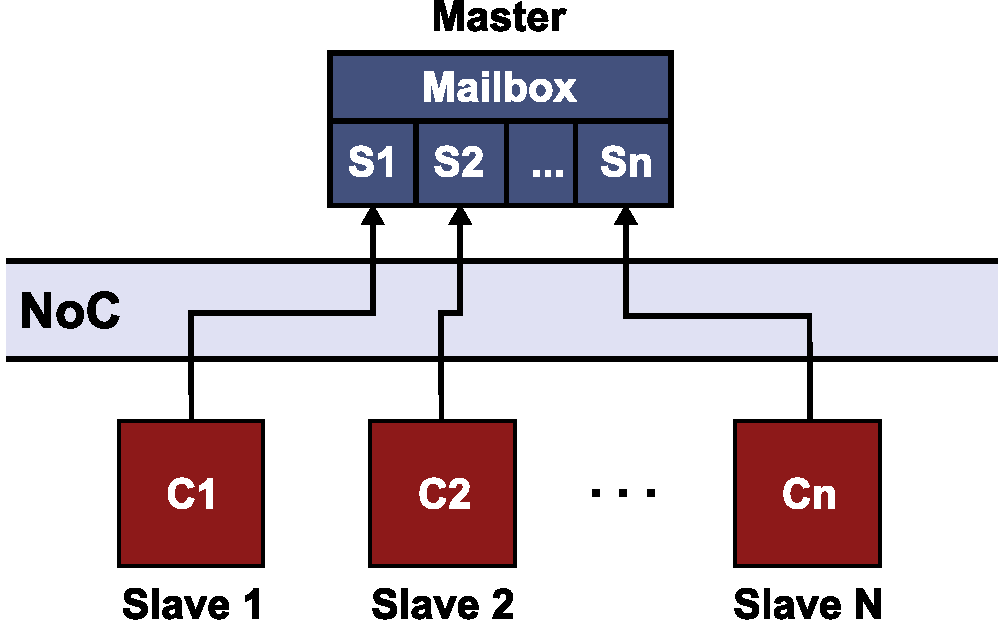
\includegraphics[width=\linewidth]{mailbox-logical.pdf}}%

					\hfill

					\subcaptionminipage[fig:conpt_mailbox-flow]%
						{.6\linewidth}%
						{Flow of execution: Slave sends a message, Master reads and notifies the sender.}%
						{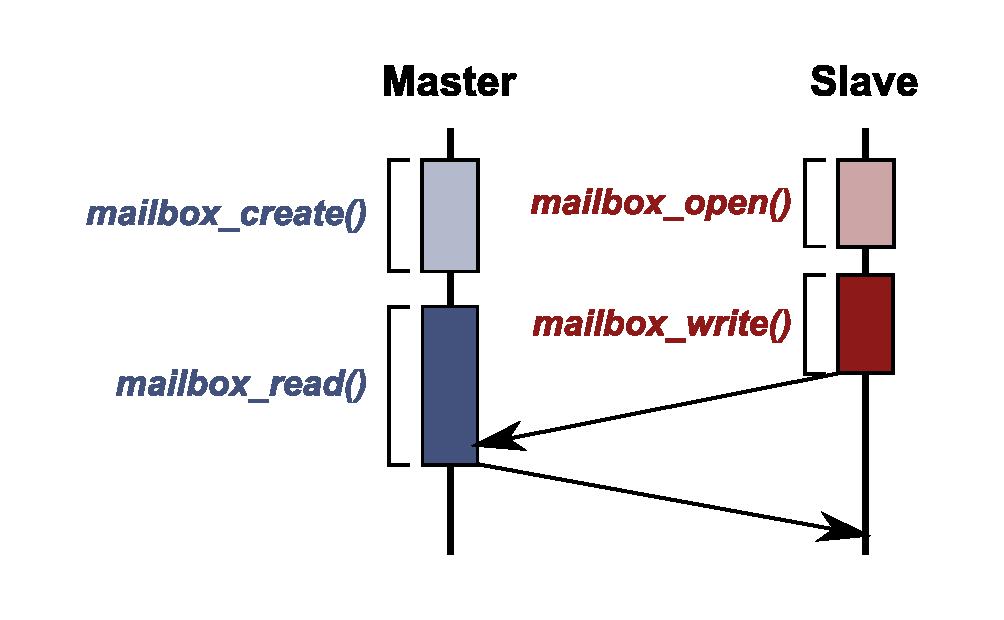
\includegraphics[width=\linewidth]{mailbox-flow.pdf}}%

					\fonte{Developed by the Author.}%
				\end{figure}

				The \textit{Mailbox Abstraction} allows clusters to exchange fixed-size
				messages with each other.
				The message was thought to be a relatively small size, usually a few hundred bytes.
				Similarly, the operation of the \mailbox follows \posix message queue behavior.
				For example, the message can be used to encode small operations and system
				control signals.
				As illustrated in \autoref{fig:conpt_mailbox}, the operation cardinality is N:1,
				where N senders can transfer one message at a time to a receiver queue.
				When the receiver consumes a message, it notifies the sender to ensure
				control of the flow.

			\subsubsubsection*{Portal Abstraction}
			\label{sec.portal-abs}

				\begin{figure}[t]
					\centering%
					\caption{Portal Abstraction Concept: Node 1 create a portal and notify Node 2 to transfer the data.}%
					\label{fig:conpt_portal}%
					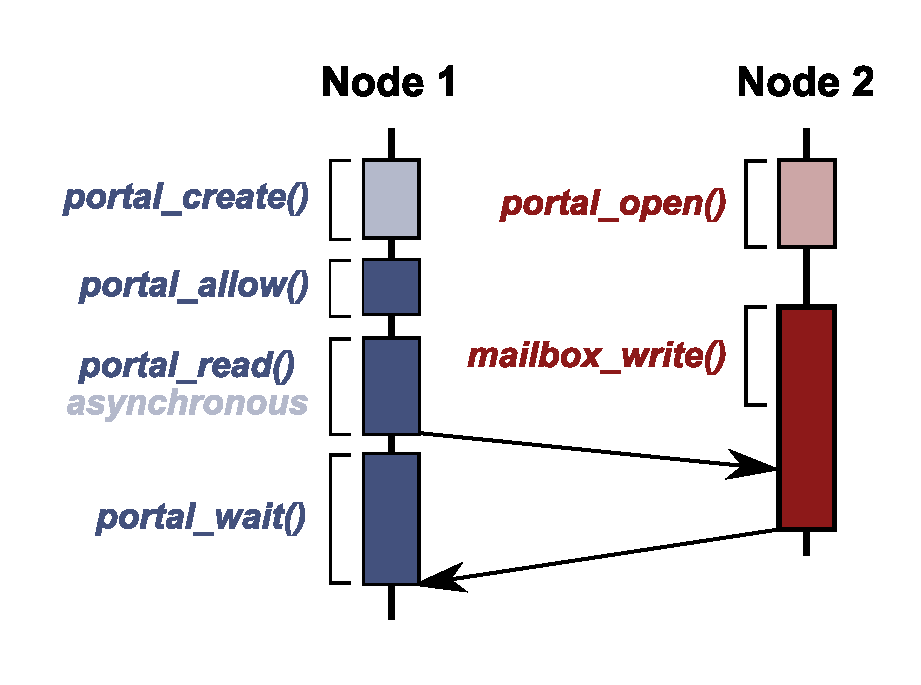
\includegraphics[width=.65\textwidth]{portal.pdf}%
					\fonte{Developed by the Author.}%
				\end{figure}

				Lastly, the \textit{Portal Abstraction} enables two clusters to exchange arbitrary
				amounts of data.
				The conceptual idea of the \portal is similar to that implemented in \posix pipes.
				\autoref{fig:conpt_portal} shows the \portal operation, with cardinality
				1:1, a cluster pair opens a channel to transfer data.
				However, the operation is only allowed in one direction with a flow control mechanism,
				where the receiver cluster warns the sender cluster when it is ready to receive.
		
	\subsection{Communication Services for the Nanvix Microkernel}
	\label{sec.communication-services}
	
		The inter-cluster communication module, described in \autoref{sec.inter-cluster-communication},
		is designed to export a standard and straightforward communication
		primitives to different lightweight manycores.
		These primitives can be used by various types of operating systems
		and applications.
		Thus, the module is flexible enough not to impact the performance
		of the upper layers negatively.
		For this, it does not provide rich management of the exposed abstractions.

		In this scenario, the communication services of Nanvix Microkernel seek
		to provide \ipc between distinct clusters.
		Specifically, these services perform the multiplexing of the hardware
		resources and the verification of the parameters that will be passed
		on the communication primitives.
		Due to the Master-Slave model, the responsibility of protecting,
		manipulating, and configuring \hal resources is of the master core.
		The slave core will request operations through a meta-interface,
		passing the necessary information to the master.

		Considering that the abstractions make up the fundamental elements of
		the construction of more complex services, the Microkernel services
		were responsible for the management and multiplexing of the finite
		resources for the many cores of a cluster.
		In total, there are three communication services in the Nanvix Microkernel,
		each associated with an abstraction of the communication module,
		analogously named \sync, \mailbox, and \portal services.

\chapter{Related Work}
\label{ch.related-work}

In this chapter, we discuss research efforts related to this
undergraduate dissertation.
First, we present an overview of the state-of-the-art on
\lightweight \manycores. Then, due to the
lack of \oss focused on lightweight manycores, we will cover
different proposed \oss for manycores in general.

\section{Lightweight Manycore Processors}
\label{sec.works.manycores}

	Several research initiatives are focused on the design of
	\lightweight \manycores, aside from the \mppa \lightweight \manycore.
	For instance, \citeonline{olofsson2014} introduce
	\epiphany as a high-performance energy-efficient \manycore
	architecture suitable for real-time embedded systems.  The
	processor features multiple nodes interconnected through three 2D mesh
	\nocs with a distributed shared-memory model without coherence
	protocol. Each node has one \risc \cpu, multi-banked local memory,
	a \dma engine, an event monitor and a network interface.  The three
	\nocs are independent, scalable, and implement a packet-switched
	model with four duplex links at every node.

	\citeonline{Wallentowitz2013} presents the open-source \optimsoc framework
	to aid manycore processor design. The \optimsoc
	enables the rapid prototyping of a manycore, either via VHDL
	simulation or \fpga synthesis.
	In this architecture, several \openrisc cores\footnote{https://opencores.org/openrisc} are bundled into
	tiles, which in turn communicate through a packet-switched \noc.
	The \noc supports various network topologies, depending only on how the tiles are disposed on chip.
	Precisely, a \textit{network adapter} handles the memory transfers between
	a tile and its local memory and provides a message-passing communication
	model among tiles.
	Tiles can communicate by using message-exchange, partitioned global
	address space without cache coherence, or global memory
	with cache coherence via a write-through policy.

	Similarly, \citeonline{Kurth2017} introduces \hero, which
	groups an \arm host processor with a fully modifiable
	\riscv \manycore implemented on an \fpga. The \pmca uses a
	multi-cluster design and relies on multi-banked memory, called \spm.
	Data transfer occurs between a local \spm and all remote \spms or
	with shared global memory. Communication to main memory passes
	through software-managed lightweight \rab. The \rab performs the
	translation of the virtual-to-physical address, similarly to
	traditional \mmu, allowing clusters to share virtual address pointers.

\section{Operating Systems for Manycores}
\label{sec.works.os}

	\citeonline{Baumann2009} proposed a new \os design for scalable multicore
	systems, called \multikernel.
	In their perspective, the next-generation of \oss should embrace the networked nature
	of the machines, and thus borrow design ideas from large-scale distributed
	systems.
	Assuming that cores are independent nodes of a network, they build traditional
	\os functionalities as fully-featured processes on userspace.
	These processes communicate via message-passing and do not share the internal
	structures of the \os.
	The work showed how expensive it is to maintain a state of the \os through
	shared-memory instead of exchanging messages and the subsequent increase of
	the complexity of cache-coherence protocols.
	The \multikernel implementation, named Barelfish, follows three design principles.
	The first principle is to \textit{make all inter-core communication explicit}, which turns the system
	amenable to human or automated analysis because processes communicate only
	through well-defined interfaces.
	The second principle is to \textit{make \os structures hardware-neutral}, so the kernel
	code can be easy to debug and optimize, facilitating the deployment of \os for new
	processor types and avoiding rework.
	The third principle is to \textit{view \os state as replicated instead of shared}, which improves system
	scalability.

	In \citeonline{Wisniewski2014}, the concept of scalability was pushed
	to the extreme, towards \hpc.
	The principal motivation is the creation of an \os that simultaneously supports
	programmability through support \linux \api, and provides a lightweight kernel
	that achieves performance, scalability, and reliability.
	The \os, named \mos, provides as much of the hardware resources as
	possible to the \hpc applications and the \linux kernel component
	acts as a service that provides \linux functionalities.

	Similarly, \citeonline{kluge2014} developed the \moosca.
	With \moosca, they introduce abstractions that are easily composed, called Nodes,
	Channels, and Servers. Nodes represent execution resources, Channels represent communication
	resources, \eg \noc resources, and lastly, Servers are nodes that provide
	services to client Nodes.
	To meet safety-critical requirements, the \manycore is partitioned and each partition
	runs replicas of Servers, turning the whole system more predictable.
	However, in order to deal with interferences in shared resources,
	usage policies were introduced to make possible the prediction of system behavior.

	Finally, \citeonline{nightingale2009} presents  Helios, aiming to
	simplify the task of writing, deploying, and optimizing an application across
	heterogeneous cores.
	They use the microkernel model, naming \textit{satellite kernel}, to export
	a uniform and straightforward set of \os abstractions.
	The most important design decisions were to avoid unnecessary remote communication
	by thinking about the penalty they have in \numa domains.
	Moreover, it requests a minimum set hardware resources to support architectures with little
	computational power or memory constraints.

\section{Discussion}

	In \autoref{sec.works.manycores}, we discussed how \manycore architectures can be
	grouped over a common logic perspective.
	They all have one or more logical units distributed and incorporated on clusters.
	The clusters, interconnected through a network, communicate by message-exchange.
	However, due to the domain for which these processors were designed, they end up
	presenting several differences among them at the hardware level.

	Additionally, \autoref{sec.works.os} presented \oss studies that focus
	on the most efficient exploration of manycores processor characteristics.
	Many of them introduce entirely new concepts, reducing the programmability
	and portability of development environments. Some even seek to provide
	\posix interfaces by porting an adapted version of known kernels, but
	this can lead to optimization losses at near-hardware levels.
	However, the \os and communication models presented fit well with the
	distributed nature of manycores.
	Finally, many of these \oss work with \numa systems,
	where a complex bus system makes communication transparent. Therefore, there
	is, in fact, no network programming. 

	In this context, \nanvix \hal offers the ground \os abstractions needed to make
	\lightweight \manycores more easy to use and program.
	The exported interfaces sought to group lightweight manycores on a common and effective view.
	Above the \hal, services will be developed that seek first and foremost
	to provide greater programmability and portability through a fully-featured
	\posix-compliant \os. \nanvix is design specifically for manycores that require explicit
	programming of communication through \noc, have
	memory constraints and miss support for cache coherency. The combination of these
	features makes designing an \os for \lightweight \manycores challenging.
\chapter{Development}
\label{ch.development}

		\todo[inline]{Need a better introducion. vvvv--- this is only copy-paste from proposal.}

	The proposal for this undergraduate dissertation is made up of two main contributions.
	The first contribution will be the port of the \textit{Inter-Cluster Communication Module},
	described in \autoref{sec.inter-cluster-communication}, for the \mppa manycore processor.
	The second contribution will be the design and implementation of communication services
	of a master-slave \os, described in \autoref{sec.communication-services}, on top of
	the inter-cluster communication module.

		\todo[inline]{Insert some paragraphs about the development, tools, etc.}

	\section{Low-Level Communication}
	\label{sec.low-level-comm}
	\todo{Or: Nanvix HAL Level}

		O Nanvix HAL provê o módulo de comunicação inter-cluster para permitir que cluster distintos troquem informações.
		Esse módulo é constituido de três abstrações, nomeados Sync, mailbox e portal.
		Essas abstrações proveêm mecânismos mais precisos, fáceis de usar, escalonáveis e facilmente portáveis para diferentes arquiteturas~\cite{wentzlaff_fleets:_2011}.
		Sobre eles, é possível criar dos mais simples serviços, como sincronização e troca de dados, à serviços mais complexos como \shm, POSIX Semaphore, \rmem~\cite{penna:rmen}.
		O comportamento esperado pode ser simulado por ambos tipos de chamadas, sincronas ou assíncronas, dependendo apenas do suporte em hardware.
		Motivados a expor melhor controle sobre QoS para as camadas superiores, nós dissociamos as pequenas transferência de dados das grandes, isto é, mailbox e portal.
		Vale notar que seria possível utilizar uma NoC para cada abstração se o hardware suportasse.
		Não fizemos isso no MPPA porque a CNoC só provê a transferência de valores de 64 bits.

		Está seção está organizada da seguinte maneira.
		Subseção 0 abrange pontos comuns entre todas as abstrações.
		Subseção 1, 2 e 3 apresentam conceitualmente cada uma das abstrações, os problemas que elas englobam, e detalhes de implementação.

		\subsection{\mppa Hardware Resources}
		\label{sec.mppa-hardware-resources}

			A realização da comunicação de baixo-nível depende principalmente de dois recursos do MPPA, interrupções e DMA.
			Primeiro, o sistema de interrupções permitirá a configuração de tratadores das mensagens recebidas e enviadas através da NoC.
			Isto possibilitará a assíncronidade das operações, ponto vital em um sistema operacional baseado no microkernel onde o mestre não pode ficar bloqueado esperando a conclusão de uma única comunicação.
			Caso não fosse possível realizar pelo menos a recebimento de dados/sinais de forma assíncrona, sérios problemas de desempenho seriam introduzidos as camadas superiores.
			Segundo, o DMA é o mediador de todas as comunicações, síncrona ou assíncronas.
			Neste ponto, um hypervisor virtualiza a DMA, separando-a em duas estruturas lógicas globais, uma para a CNoC e outra para a DNoC.
			Cada estrutura agrupa os registradores para a configuração de envio/recebimento, e campos de bits indicando quais slots geraram uma interrupção.
			O hypervisor executa nos RM e controla, de forma assíncrona, as permissões de leitura/escrita dos registradores virtualizados.

			O controle efetuado pelo hypervisor não engloba a alocação ou manipulação dos recursos.
			Consequentemente, nós controlamos manualmente a alocação através de campos de bits.
			Caso uma operação não esteja em conformidade com esse controle, é retornado um valor negativo indicando o erro, \eg alocação de um recursos que já está em uso.
			Assim, não inflingimos custos indesejados ao transferir a responsabilidade de tratar o erro a camada superior, \eg aguardar a liberação do recurso.
			A manipulação envolve procedimentos para configurar a DMA com as devidas permissões e garantir a coerência de cache das operações.
			Por fim, vale ressaltar que não é realizado nenhum controle de concorrência sobre as estruturas comentadas para que não seja inflingido um sobre custo sobre a abordagem do microkernel.
			Caso a HAL seja utilizada para desenvolver um sistema operacional monolítico, o mesmo deve se preocupar em garantir a atômicidade das operações.

			A DMA coordena três linhas de interrupções.
			Duas delas são utilizados pela DNoC para notificar o recebimento de dados e o término do envio dados por uma microthread.
			A CNoC só utiliza uma linha para o recebimento de sinais porque o envio de um sinal, um valor de 64-bits, é realizado explicitamente pelo core.
			Para cada linha de interrupção existe um handler específico mas todos executam um algoritmo similar.
			O Algoritmo 3 exemplifica de forma simplificada o comportamento de um handler.
			Devido ao fato que a linha apenas notifica qual o tipo de interrupção, é responsabilidade do manipulador varrer os recursos de cada interface procurando quem acionou a interrupção.
			Para que não ocorresse a perda de interrupções, foi garantido que o manipulador fosse reentrante.
			Devido ao abordagem do microkernel, os problemas de concorrência são amenizados porque apenas o mestre trata as interrupções.

			\begin{algorithm}
				\caption{Simplified NoC Handler Algorithm.}%
				\label{alg.noc-handler}%
				\begin{algorithmic}[1]
					\Require $status[M_{Interfaces}][N_{Resources}]$, interrupt status of a resource.
					\Require $handlers[M_{Interfaces}][N_{Resources}]$, interrupt handler of a resource.
					\Procedure{noc\_handler}{}
					\For {$i \in [1, M_{Interfaces}]$}
						\For {$j \in [1, N_{Resources}]$}
							\If {$status[i][j] == Interrupt Triggered$}
								\State {$\Call{clean\_status}{i, j}$}
								\State {$\Call{handlers[i][j]}{i, j}$}
							\EndIf
						\EndFor
					\EndFor
					\EndProcedure
				\end{algorithmic}%
				\fonte{Developed by the Author.}%
			\end{algorithm}

			NoC interfaces have two identifiers, one physical (physical ID) and the other logical (logical ID).
			The hardware uses the physical IDs in the process of data routing through \noc.
			Each physical ID is associated with a Logical ID to enable the identification
			of \noc nodes outside the \hal.
			Logical IDs primarily serve to disassociate the node identification from the
			architecture that implements the \hal.
				\autoref{tab.noc-node-id} shows the physical and logical identification performed for \mppa.
			A Tabela 3 apresenta o mapeamento proposto para os clusters do MPPA.
			Cada linha apresenta um dos três grupos de nós NoC existentes (primeira coluna), agrupados por proximidade dos identificadores lógicos.
			Dentro de cada grupo temos um conjunto de identificadores físicos (segunda coluna) que são mapeados 1 para 1 para os identificadores lógicos (terceira coluna).
			Por exemplo, o grupo IO0 constitui 4 interfaces, onde são mapeadas da seguinte forma: $128 \to 0$, $129 \to 1$, $130 \to 2$, e $131 \to 4$.
			A ordem do mapeamento foi definido desta maneira para ficar mais intuitivo qual das interfaces, por consequência o cluster, é o mestre.
			Neste caso, o nó mestre é o identificador lógico 0, IO0.
			Este processo facilita na sincronização após o boot.

			\begin{table}[!tb]
				\centering%
				\caption{NoC Interface Identification.}%
				\label{tab.noc-node-id}%

				\begin{tabular}{l|l|l|}
					\cline{2-3}
															& \textbf{Physical ID} & \textbf{Logical ID} \\ \hline
					\multicolumn{1}{|l|}{\textbf{\iocluster0}} & 128-131              & 0-3                 \\ \hline
					\multicolumn{1}{|l|}{\textbf{\iocluster1}} & 192-195              & 4-7                 \\ \hline
					\multicolumn{1}{|l|}{\textbf{\ccluster}}   & 0-15                 & 8-23                \\ \hline
				\end{tabular}

				\fonte{Developed by the Author.}%
			\end{table}

			Para performar a comunicação entre dois clusters, é necessário que o emissor conheça qual o identificador do recurso que o receptor irá usar.
			Por exemplo, caso o receptor configurar o recebimento em um recurso da DNoC e o emissor enviar para outro, mesmo que o identificador lógico esteja correto, o receptor não será notificado do recebimento.
			Por esta razão, os slots de recebimento da CNoC e DNoC foram particionados por abstração.
			Dentro de uma partição, cada slot é mapeado estaticamente para um identificador lógico, \eg 0 à 23.
			Em contraste, os canais de envio não possuem essa necessidade, podendo ser alocados dinâmicamente.
			Entretanto, um conceito importante do Nanvix HAL é prover os recursos necessários para uma determinada operação sem realizar otimizações desnecessárias.
			Desta forma, os canais de envio também foram particionados por abstração de modo que sejam reservados durando toda uma operação.
			A tabela 3 apresenta cada abstração, identificados pelas linhas, e o particionamento dos recursos de cada NoC, identificados pelas colunas.
			Como a abstração sync não realiza a troca de dados arbitrários, não foram reservados recursos na DNoC.
			Vale notar que mesmo com a não utilização de todos os slots existentes, o aperfeiçoamento da programabilidade por não necessitar especificar os recursos de uma comunicação é um ponto forte do design das abstrações.

			% To perform the communication between two clusters, it is necessary that the
			% sender knows which resource the receiver will use.
			% For this reason, the receive slot range of \cnoc and \dnoc are partitioned
			% by abstraction, as can be seen in \autoref{tab.noc-resources}.
			% Within a partition, each slot is associated with a cluster's logical ID.
			% 	\todo{"On the another hand" does not make sense AGAIN.}
			% On the other hand, the transmitters use sending channels that need to
			% be reserved during the entire operation.
			% 	\todo{Explain the table.}
			% Thus, \autoref{tab.noc-resources} also shows the partition of the
			% sending channels for each abstraction.

			\begin{table}[!tb]
				\centering%
				\caption{Partitions of NoC resources by abstraction.}%
				\label{tab.noc-resources}%

				\todo[inline]{Explicar a motivação na separação dos recursos. Por que o portal tem 2 cnoc tx?}

				\begin{tabular}{l|l|l|l|l|}
					\cline{2-5}
															& \multicolumn{2}{c|}{\textbf{\cnoc}}          & \multicolumn{2}{c|}{\textbf{\dnoc}}          \\ \cline{2-5}
															& \textbf{RX Slot ID} & \textbf{TX Channel ID} & \textbf{RX Slot ID} & \textbf{TX Channel ID} \\ \hline
					\multicolumn{1}{|l|}{\textbf{\mailbox}} & 0-23                & 0                      & 0-23                & 1-3                    \\ \hline
					\multicolumn{1}{|l|}{\textbf{\portal}}  & 24-47               & 1-2                    & 24-47               & 4-7                    \\ \hline
					\multicolumn{1}{|l|}{\textbf{\sync}}    & 48-71               & 3                      & -                   & -                      \\ \hline
				\end{tabular}

				\fonte{Developed by the Author.}%
			\end{table}

			Por fim, nós conseguimos remover quase toda dependência com a pilha de software disponibilizada pela Kalray.
			Porém, ao eliminar as biliotecas de comunicação, a falta de documentação da virtualização do hardware e exemplos funcionais de comunicação, surgiram limitações no envio dos dados pela DNoC.
			Resumidamente, não foi possível configurar corretamente as microthreads existentes na DMA para envio assíncrono, tornando-se um trabalho futuro.
			Entretanto, tal limitação não impactou no design das abstrações exigindo apenas que o core mestre perca um tempo enviando os dados manualmente.

		\subsection{General Concepts of Communication Abstractions}
		\label{sec.general-concepts}

			Tecnicamente, o Nanvix HAL não sabe que tipos de aplicações ou kernels o utilizaram.
			Desta forma, é preciso garantir um comportamento comum que não afete o funcionanto da camada superior.
			O microkernel, especificamente, restringe o core mestre a estar quase sempre disponível para atender solicitações dos escravos.
			Por isso, as interfaces exportam apenas chamadas assíncronas (isto é, funções async e wait).
			Isto força a camada superior, caso queira, criar chamadas síncronas que chamam a função wait logo após a operação assíncrona.
			Deste modo, no nível do microkernel, nós conseguimos garantir que o mestre configure ou execute as funções assíncronas e notifique os escravos que aguardam na função wait.
			No MPPA, este controle é realizado através de spinlocks atrelados a cada recurso das abstrações.
			Ao concluir uma operação, o mestre libera o bloqueio para o escravo continuar sua execução.

			Contudo, a limitação da DMA descrita na Seção 0 acrescenta um agravante na operação de transferência das abstrações mailbox e portal.
			Nestas abstrações, existe um controle de fluxo onde o receptor deve notificar o emissor, dando-lhe permissão para transferir os dados.
			Este comportamento pode ocasionar o bloqueio do mestre ao esperar uma permissão.
			Para burlar esse problema, foi introduzido o conceito de envio preguiçoso.
			O algoritmo 4 ilustra o comportamento do envio preguiçoso, onde o mestre guarda os paramêtros caso não tenha permissão e vai atender outras solicitações.
			Ao receber a permissão do receptor, o manipulador de interrupções identifica o recurso, realiza de fato o envio dos dados e libera o escravo que solicitou o envio.
			Assim, nós garantimos que o mestre deixe de fazer algo útil e trave todo o sistema.

			\begin{algorithm}
				\caption{Simplified Lazy Transfer Algorithm.}%
				\label{euclid}%
				\begin{algorithmic}[1]
				\Require $resources$, Abstraction Resource Table

				\Algphase{Configures data transfer.}

					\Procedure{async\_write}{$id, message, size$}
						\State {$resources[id].message \gets message$}
						\State {$resources[id].size \gets size$}
						\If {$resources[id].has\_permission$} 
							\State {$\Call{do\_lazy\_write}{id}$}
						\Else
							\State {$resources[id].is\_waiting \gets True$}
						\EndIf
					\EndProcedure%

				\Algphase{Receives permission.}

					\Procedure{abstraction\_handler}{$id$} 
						\If {$resources[id].is\_waiting$} 
							\State {$\Call{do\_lazy\_write}{id}$} 
						\Else
							\State {$resources[id].has\_permission \gets True$}
						\EndIf
					\EndProcedure%

				\Algphase{Transfers the data.}

					\Procedure{do\_lazy\_write}{$id$} 
						\State {$resources[id].is\_waiting \gets False$}
						\State {$resources[id].has\_permission \gets False$}
						\State {$\Call{transfer\_data}{resources[id].message, resources[id].size}$} 
						\State {$\Call{unlock}{resources[id].lock}$}                                \Comment{Releases slave core.}
					\EndProcedure%

				\end{algorithmic}%

				\fonte{Developed by the Author.}%
			\end{algorithm}

			Por fim, as interfaces das abstrações seguem uma convenção para distinguir os papeis de receptor e emissor.
			Receptores utilizam as funções com sufíxo \texttt{create}, \texttt{unlink}, \texttt{aread} e \texttt{wait}.
			Emissores, por sua vez, utilizam funções com sufíxo \texttt{open}, \texttt{close}, \texttt{awrite} e \texttt{wait}.
			Como a função \texttt{wait} é compartilhada, a abstração deve fazer a distinção do papel pelo identificador do recurso.
			A diferenciação da natureza das operações ajuda tanto o usuário, sendo bastante intuitivo, como na implementação da HAL por explicitar quais recursos serão necessário.

			% Por fim, como já comentado anteriormente, o Nanvix HAL não realiza nenhum tipo de multiplexação dos recursos físicos do hardware.
			% A quantidade de recursos de comunicação disponíveis é diretamente relativa a quantidade de recursos físico para realizar uma dada operação.
			% A tabela 4 mostra quais recursos físicos são necessário para cada abstração e a quantidade total de abstrações simultaneas que podem existir.
			% Por exemplo, a criação de um portal precisa de um slot de recebimento da DNoC e 1 canal de transmissão da CNoC.
			% As quantidades são baixas devido aos poucos canais de transmissão, porém quem deve se preocupar com a multiplexação dos recursos deve ser da camada superior.

			% \begin{table}[!tb]
			% 	\centering%
			% 	\caption{Physical requirements by abstraction.}%
			% 	\label{tab.abstractions-amount}%

			% 	\begin{tabular}{l|l|l|l|l|l|l|}
			% 		\cline{2-7}
			% 												& \multicolumn{3}{c|}{\textbf{Create}}  & \multicolumn{3}{c|}{\textbf{Open}}                              \\ \cline{2-7}
			% 												& \multicolumn{1}{|c|}{\textbf{RX}}
			% 												            & \multicolumn{1}{|c|}{\textbf{TX}}
			% 															            & \multicolumn{1}{|c|}{\textbf{Available}}
			% 																		                & \multicolumn{1}{|c|}{\textbf{RX}}
			% 																				                    & \multicolumn{1}{|c|}{\textbf{TX}}
			% 																				        			            & \multicolumn{1}{|c|}{\textbf{Available}} \\ \hline
			% 		\multicolumn{1}{|l|}{\textbf{\mailbox}} & 1 (\dnoc) & 1 (\cnoc) & 1             & 1 (\cnoc) & 1 (\dnoc) & 4                                        \\ \hline
			% 		\multicolumn{1}{|l|}{\textbf{\portal}}  & 1 (\dnoc) & 1 (\cnoc) & 2             & 1 (\cnoc) & 1 (\dnoc) & 4                                        \\ \hline
			% 		\multicolumn{1}{|l|}{\textbf{\sync}}    & 1 (\cnoc) & 0         & 24            & 0         & 1 (\cnoc) & 1                                        \\ \hline
			% 	\end{tabular}

			% 	\fonte{Developed by the Author.}%
			% \end{table}

		\subsection{Sync Abstraction}
		\label{sec.sync-abs}

			A abstração de sincronização, chamada sync, provê o básico para a sincronização de clusters.
			A partir dela, é possível criar barreiras distribuidas.
			Seu comportamento é análogo a abstração POSIX Signals, mas as notificações não carregam informações, servem apenas para sincronização.
			O sync define dois modos de sincronização, ALLTOONE e ONETOALL.
			Nois dois modos, os clusters são separados entre um único nó mestre (ONE) e um ou mais nós escravos (ALL).
			A Figura 1 ilustra o modo ALLTOONE, onde o nó mestre aguarda bloqueado os N escravos realizarem a sincronização.
			Em contrapartida, o modo ONETOALL é utilizado quando o mestre notifica os N escravos, liberando-os do bloqueio, ilustrado pela Figura 3.
			Os nós emissores nunca ficam bloqueados, o trabalho deles é emitir um sinal.
			Os nós receptores são responsáveis por aguardar a chegada de todas as notificações.

			\begin{figure}[!tb]
				\centering%
				\caption{Synchronization Abstraction Example.}%
				\label{fig:sync-concepts}%

				\subcaptionminipage[fig:sync-all-to-one]%
					{.6\linewidth}%
					{N Slaves notify the Master (\texttt{ALL\_TO\_ONE}).}%
					{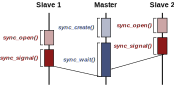
\includegraphics[width=\linewidth]{sync-all-to-one.pdf}}%
				\hfill
				\subcaptionminipage[fig:sync-one-to-all]%
					{.6\linewidth}%
					{The Master notify N Slaves (\texttt{ONE\_TO\_ALL}).}%
					{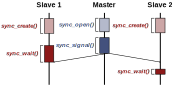
\includegraphics[width=\linewidth]{sync-one-to-all.pdf}}%

				\fonte{Developed by the Author.}%
			\end{figure}

			\subsubsection{Receiver Side Implementation}

% O que é a interface?
% Quais são os parâmetros para realizar uma operação?
				O Codigo 4 apresenta a interface Sync para nós receptores proposta para o Nanvix HAL.
				Os parâmetros necessário para a abertura de um ponto de sincronização é uma lista de IDs lógicos, o tamanho da lista e o tipo de sincronização.
				A lista deve ser sempre inicializada com o ID do nó mestre, independentemente do modo.
				Os identificadores restantes, contando que não tenham repetição, podem estar em qualquer ordem.
				O tipos de sincronização são os modos descritos anteriormente definidos através de constantes.
				As demais funções utilizam o identificador da abstração retornado pela função de criação.
				Caso algum parâmetro esteja em desacordo ou inválido, um valor negativo é retornado indicando o erro, \eg, \texttt{nodes == NULL}.

\begin{listing}[!tb]
\caption{Nanvix HAL: Sync Interface for Receiver Node.}
\label{code:hal-sync-receiver}
\begin{minted}{c}
/**
 * @brief Allocates and configures the receiving side of
 * the synchronization point.
 */
int sync_create(const int *nodes, int nnodes, int type);

/* @brief Releases and cleans receiver slot. */
int sync_unlink(int syncid);

/* @brief Waits a signal. */
int sync_wait(int syncid);
\end{minted}
\fonte{Developed by the Author.}
\end{listing}

% Quais recursos são necessário para cada tipo de operação, envio e recebimento?
				O recebimento das notificações requer a reserva 1 slot rx da CNoC relativo ao identificador do mestre.
				Deste modo, eliminamos o conflito no uso de diferentes slots por diferentes configurações de sincronização.
				Em contrapartida, um nó não poderá ser o mestre em duas operações simultâneas.
				O total de abstrações que podem ser criadas desta maneira é igual a quantidade de nós existentes (24 no MPPA).
				Nos cluster I/O, este total é multiplicado pelo número de interface NoC disponíveis, ou seja, 24 por DMA.
				A configuração do slot é realizado através de uma máscara de 64-bits.
				Está mascará é construida com os IDs lógicos dos emissores de modo que os bits relativos a suas posições sejam iguais a 0.
				Ao receber um sinal, a DMA realiza um OR com o valor anterior.
				Quando todos os bits se tornarem 1's, a DMA zera todos os bits do registrador e emite uma interrupção.

% Como as operações funcionam?
				Um vetor de estruturas internas realiza o controle das operações.
				Cada posição do vetor é reservado a um slot físico e guarda flags de controle, a mascará e um spinlock.
				Ao realizar a abertura, espera ou unlink de um sync, a HAL verifica discrepâncias nos IDs, nas flags de controle ou nos parâmetros.
				Por fim, o spinlock é utilizado para sincronização da operação com os núcleos escravos.
				Em um sistema microkernel, o core mestre configura o sync e o escravo aguarda ser liberado no spinlock.
				O tratador de interrupções do Sync identifica a estrutura e libera o bloqueio.
				A falta de coerência de cache não afeta os spinlock porque são utilizadas instruções que garantem a atomicidade que implementam o lock.

% Como foi resolvido o problema de multiplos nós nos IOs? PRECISA FALAR? DARIA PRA ARRUMAR ISSO NO CÓDIGO FORÇANDO QUE O ID[1] FOSSE O ID LOCAL (CASO NAO FOR O MESTRE).
				% A lista de nós foi projetada para utilizar os IDs das interfaces NoCs ao invés dos IDs dos Cluster para não desperdiçar as DMAs extras existentes nos Cluster I/O.

			\subsubsection{Sender Side Implementation}

% O que é a interface?
% Quais são os parâmetros para realizar uma operação?
				A interface do nó emissor, apresentada pelo Código 3, utiliza os mesmo parâmetros para abertura de um sync.
				Ao utilizar os mesmo valores na criação e abertura, a aplicação cliente pode definir o papel do cluster simplemente definindo qual função deve ser chamada.
				Entretanto, tanto na criação quanto na abertura, o ID lógico local deve estar Range correto do lista.
				Por exemplo, um sync é aberto com o ID local como mestre mas o tipo de sincronização é definido como ALL\_TO\_ONE.
				Isto retornará um erro e o sync não será aberto porque o mestre deveria ser o receptor das notificações e não o emissor.
				O restante da implementação segue o que já foi explicado na seção anterior.

\begin{listing}[!tb]
\caption{Nanvix HAL: Sync Interface for Sender Node.}
\label{code:hal-sync-sender}
\begin{minted}{c}
/**
 * @brief Allocates and configures the sending side of
 * the synchronization point.
 */
int sync_open(const int *nodes, int nnodes, int type);

/* @brief Releases the transfer channel. */
int sync_close(int syncid);

/* @brief Sends a signal. */
int sync_signal(int syncid);
\end{minted}
\fonte{Developed by the Author.}
\end{listing}

% Quais recursos são necessário para cada tipo de operação, envio e recebimento?
				De maneira oposta ao receptor, o emissor necessita de 1 canal de envio da CNoC para abrir um sync.
				Devido a separação dos canais descritos na seção (MPPA HARDWARE), um nó só poderá abrir um sync por vez.
% Como as operações funcionam?
				Para emitir um sinal, o nó precisa identificar o ID lógico e o slot de recebimento do mestre.
				A mascará que será ser enviada é sempre um valor de 64-bits com o bit relativo ao nó emissor setado como 1.
				A estrutura de controle do emissor também possui flags para garantir a semântica das operações.
				Somado a isso, o emissor guarda, em um array de inteiros, todos os IDs lógicos dos destinatário do sinal.
				Ao performar de fato o envio, será configurado e enviado um sinal para cada target desta lista.
				O envio do sinal é realizado através da escrita em um registrador da DMA, desta maneira, não é possível realizar esta ação de forma assíncrona como as demais abstrações.

		\subsection{Mailbox Abstraction}
		\label{sec.mailbox-abs}


			% The \textit{Mailbox Abstraction} allows clusters to exchange fixed-size
			% messages with each other.
			% The message was thought to be a relatively small size, usually a few hundred bytes.
			% Similarly, the operation of the \mailbox follows \posix message queue behavior.
			% For example, the message can be used to encode small operations and system
			% control signals.
			% As illustrated in \autoref{fig:mailbox}, the operation cardinality is N:1,
			% where N senders can transfer one message at a time to a receiver queue.
			% When the receiver consumes a message, it notifies the sender to ensure
			% control of the flow.

			A abstração \textit{Mailbox} permite que clusters troquem mensagens
			de tamanho fixo entre si.
			O tamanho da mensagem foi projetado para ser relativamente pequeno,
			geralmente algumas centenas de bytes.
			Essas mensagens são consumidas pelo receptor sem a necessidade de conhecer quem as enviou.
			Similarmente, a operação da \mailbox segue o comportamento da fila de mensagens \posix.
			A Figura (conceito) ilustra conceitualmente uma das formas de implementar uma Mailbox.
			O receptor aloca espaço suficiente para receber 1 mensagem de cada possível emissor.
			O emissor envia para o espaço reservado para sua mensagem, eliminando a concorrência de escrita das mensagens.

			\begin{figure}[!tb]
				\centering%
				\caption{Mailbox Abstraction Concept.}%
				\label{fig:mailbox}%

				\subcaptionminipage[fig:mailbox-concept]%
					{.4\linewidth}%
					{Conceptual Overview.}%
					{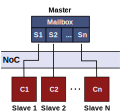
\includegraphics[width=\linewidth]{mailbox-concept.pdf}}%

				\hfill

				\subcaptionminipage[fig:mailbox-flow]%
					{.5\linewidth}%
					{Flow of execution: Slave sends a message, Master reads and notifies the sender.}%
					{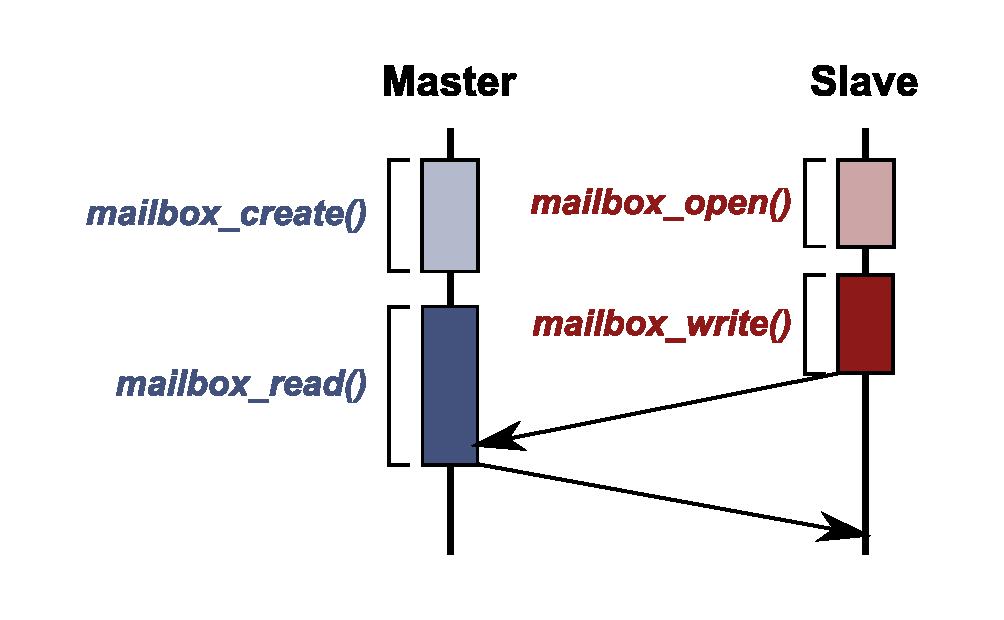
\includegraphics[width=\linewidth]{mailbox-flow.pdf}}%

				\fonte{Developed by the Author.}%
			\end{figure}

			A Figura (fluxo) exemplifica o fluxo de comunicação entre um nó receptor e um emissor.
			A criação de uma Mailbox cria uma fila de mensagens vazia, onde os emissores são livres para enviar a primeira mensagem.
			Posteriormente, todos os envios necessitaram da permissão do receptor para que mensagens não sejam sobreescritas.
			Por este motivo, o receptor notificará o emissor ao consumir sua mensagem.
			A mensagem será copiada para um buffer do usuário e o espaço estará novamente disponível.

			Teoricamente, a quantidade de mensagens permitidas por emissor pode ser de 1 à N.
			Entretanto, optou-se por permitir apenas 1 no Nanvix HAL devido as restrições de memória apresentada por manycores.
			E como o espaço é alocado estatícamente dentro do espaço de memória do kernel, permitir que o usuário escolhe-se o tamanho da fila de mensagem não reduziria o espaço prévio necessário.
			Todavia, o uso de uma mensagem é suficiente para programas servidores tratarem requisitações no nível do Multikernel.
			Por exemplo, a mensagem pode ser usada para codificar pequenas operações e sinais de controle do sistema.

			\subsubsection{Receiver Side Implementation}

% Interface e seus parâmetros
				O código 3 apresenta a interface da Mailbox para um nó receptor.
				A criação de uma Mailbox requer que a aplicação informe o ID Lógico no nó local.
				Esta identificação é necessária por causa do múltiplos nós existentes nos Cluster I/O.
				As demais operações utilizam o identicador retornado na criação da mailbox.
				Para a leitura de uma mensagem, o usuário é obrigado a passar o local onde a mensagem será copiada e o tamanho a ser copiado.
				O tamanho é sempre constante mas é utilizado como verificação da integridade da operação.
				A cópia bem sucedida de uma mensagem liberará o escravo que executar a função de espera.
				Neste processo de liberação, o core mestre executa o flush da mensagem para a SRAM para que o escravo, ao invalidar a sua cache, possa ler a mensagem.

% Recursos de hardware
				A Mailbox é mais complexa do que o Sync porque utiliza recursos DNoC e CNoC.
				Especificamente, o receptor necessita de 1 slot de recebimento da DNoC e 1 canal de transmissão da CNoC.
				A necessidade de 1 canal de transmissão durante toda a vida da Mailbox do receptor limita a criação de apenas 1 mailbox por nó NoC.
				O slot rx é configurado utilizando dois tamanhos.
				Um para o tamanho de uma mensagem, o qual gerará interrupções, e outro para o tamanho total buffer alocado para proteção.
				O buffer é alocado dentro da memória do kernel com espaço suficiente para receber 24 mensagens.
				A mensagem, propriamente dita, é composta por um cabeçalho identificando o emissor, um corpo contendo a mensagem útil e um rodapé com o mesmo identificador.
				O canal de transmissão, por sua vez, é utilizado após a cópia da mensagem útil para o buffer do usuário, notificando o ID do cabeçalho.

% Desafios da implementação
				O paralelismo no recebimento das mensagens introduziu alguns desafios na leitura assíncrona do Mailbox como 
				(i) cada mensagem gera uma interrupção,
				(ii) interrupções preemptadas por outras não encontraram os recursos da DNoC que emitiram a interrupção e
				(iii) não é possível verificar a quantidade de interrupções geradas por um recurso.
				Para burlar estas barreiras, foi implementado um comportamento similar ao envio preguiçoso.
				Primeiro, um contador global contendo a quantidade total de mensagens recebidas permite que o receptor copie mensagens recebidas antes de uma leitura.
				Segundo, caso não haja mensagens disponíveis, a cópia será realizada pelo próximo disparo do manipulador.
				Terceiro, para resolver o problema das interrupções preemptadas, sempre que um manipulador é disparado ele percorrerá a fila de mensagens conferindo os cabeçalhos e rodapés.
				Ao identificar uma mensagem válida, o manipulador incrementa o contador e altera o rodapé para um código especifico.
				Desta forma, não perdemos nenhuma mensagem por não tratar uma interrupção.

\begin{listing}[!tb]
\caption{Nanvix HAL: Mailbox Interface for Receiver Node.}
\label{code:hal-mailbox-receiver}
\begin{minted}{c}
/* @brief Creates a mailbox. */
int mailbox_create(int nodenum);

/* @brief Destroys a mailbox. */
int mailbox_unlink(int mbxid);

/* @brief Reads data asynchronously from a mailbox. */
ssize_t mailbox_aread(int mbxid, void * buffer, size_t size);

/* @brief Waits for an asynchronous operation to complete. */
int mailbox_wait(int mbxid);
\end{minted}
\fonte{Developed by the Author.}
\end{listing}

			\subsubsection{Sender Side Implementation}

% Interface e seus parâmetros
				O código 3 apresenta a interface da mailbox para o nó emissor.
				A abertura de uma mailbox requer que a aplicação informe o ID lógico do nó que irá receber a mensagem.
				O identificador da mailbox retornado pela função de abertura é utilizada para configurar e controlar as demais funções.
				A função de envio, em especial, implementa o conceito de envio preguiçoso.
				Ou seja, o core mestre nunca ficará bloqueado caso a mailbox não tenha permissão para enviar a mensagem.
				Ele realiza o agendamento do envio setando valores nas estruturas internas do kernel e copiando a mensagem útil para um buffer local, no qual consta o identificador do emissor.
				A função de espera é a mesma função utilizada pelo nó receptor onde o núcleo escravo aguardaram bloqueado em um spinlock até receber a permissão de envio.

				% If the sender attempts to send a message before the receiver has consumed
				% the previous message, the sender will be blocked waiting for the sender's notification.
				% In this way, flow control is guaranteed, and the sender will not overwrite
				% messages unread by the receiver.

\begin{listing}[!tb]
\caption{Nanvix HAL: Mailbox Interface for Sender Node.}
\label{code:hal-mailbox-sender}
\begin{minted}{c}
/* @brief Opens a mailbox. */
int mailbox_open(int nodenum);

/* @brief Closes a mailbox. */
int mailbox_close(int mbxid);

/* @brief Writes data asynchronously to a mailbox. */
ssize_t mailbox_awrite(int mbxid, const void * buffer, size_t size);

/* @brief Waits for an asynchronous operation to complete. */
int mailbox_wait(int mbxid);
\end{minted}
\fonte{Developed by the Author.}
\end{listing}

% Recursos de hardware
				O lado emissor também exige a alocação de recursos das duas NoCs.
				Porém, os recursos são opostos ao do receptor, no qual serão alocados 1 slot rx da CNoC e 1 canal de transmissão da DNoC.
				O slot rx CNOC alocado é relativo ao ID do receptor para evitar que aberturas para receptores distintos conflitassem ao tentar alocar o mesmo slot.
				O canal de transmissão é alocado dinamicamente dentre os 4 disponíveis.
				Deste modo, a quantidade máximo de mailboxes abertas por nó é limitado pelo número de canais de transmissão.

		\subsection{Portal Abstraction}
		\label{sec.portal-abs}

			% \begin{figure}[!tb]
			% 	\centering%
			% 	\caption{Portal Abstraction Concept: Node 1 create a portal and notify Node 2 to transfer the data.}%
			% 	\label{fig:portal}%
			% 	\includegraphics[width=.65\textwidth]{.pdf}%
			% 	\fonte{Developed by the Author.}%
			% \end{figure}

% Apresentação do portal e o conceito.
			Por fim, a abstração Portal permite que dois nós troquem quantidades arbitrárias de dados.
			A Figura (conceito) apresenta a ideia conceitual do portal, onde se assemelha a do POSIX Pipes com controle de fluxo.
			A cardinalidade das operações é sempre 1:1, onde um par de nós abre um canal unidirecional para transferência de dados.
			Porém, ao contrário do POSIX Pipes que define que o pipe existe apenas entre dois processos, o portal permite que o receptor se comunique com outros nós através de um mesmo canal.
			O emissor, por sua vez, poderá apenas se comunicar com um nó.

% Fluxo da operação
			A Figura (fluxo) exemplifica o controle de fluxo proposto para o portal.
			Ao tentar transmitir dados ao receptor, o emissor blorqueará até que o receptor esteja apto à receber.
			O receptor, ao habilitar uma troca de dados de cada vez, configura a leitura e notifica o emissor.
			Deste modo, o controle de fluxo garante que o receptor não será sobrecarregado, não receberá dados sem que a DMA esteja devidamente configurada, e não sobrescreverá dados prévios.
			O ato de habilitar uma comunicação permite que o receptor escolha com qual nó deseja se comunicar.

% Diferença do posix, receptor allows multiples issuers

			\begin{figure}[!tb]
				\centering%
				\caption{Portal Abstraction Concept.}%
				\label{fig:portal}%

				\subcaptionminipage[fig:portal-concept]%
					{.4\linewidth}%
					{Conceptual Overview.}%
					{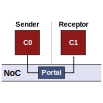
\includegraphics[width=\linewidth]{portal-concept.pdf}}%

				\hfill

				\subcaptionminipage[fig:portal-flow]%
					{.5\linewidth}%
					{Node 1 create a portal and notify Node 2 to transfer the data.}%
					{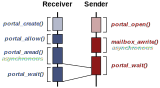
\includegraphics[width=\linewidth]{portal-flow.pdf}}%

				\fonte{Developed by the Author.}%
			\end{figure}

			\subsubsection{Receiver Side Implementation}

% Interface e seus parâmetros
				O Código 5 apresenta a interface portal para nós receptores.
				Assim como a mailbox, a aplicação deve identificar o nó local para criar um portal.
				As demais funções utilizam o identificador do portal retornado pela função de criação.
				Para criar um canal de comunicação, o receptor sempre deverá executar 3 operações, allow, aread, wait.
				A função allow aloca um slot rx relativo ao nó remoto informado, limitando um canal por par de nós.
				Entretanto, a notificação apenas será enviada, relativo ao nó remote, após a configuração da DMA pela função aread.
				Por fim, o nó bloqueará na função wait até a comunicação ser completada.

% Recursos de hardware
				Um portal receptor aloca um slot rx da DNoC e um canal tx da CNoC.
				Diferente da mailbox, o portal tem disponível 2 canais tx o que permite a criação de dois portais simultâneos.
				Tais portais não podem se comunicar com o mesmo nó ao mesmo tempo por causa da escolha do slot físico da DMA comentado no parágrafo anterior.
				A leitura configura o slot rx com o buffer e tamanho informado pela aplicação.
				Isto elimina as cópias intermediárias como da mailbox, onde a DMA escreve os dados direto no buffer da aplicação.
				As estruturas de controle também são simplificadas por causa disso
				contendo apenas flags e um spinlock liberado pelo manipulador do portal.

\begin{listing}[!tb]
\caption{Nanvix HAL: Portal Interface for Receiver Node.}
\label{code:hal-portal-receiver}
\begin{minted}{c}
/* @brief Creates a portal. */
int portal_create(int local);

/* @brief Destroys a portal. */
int portal_unlink(int portalid);

/* @brief Allow sender to transfer data. */
int portal_allow(int portalid, int remote);

/* @brief Reads data asynchronously from a portal. */
ssize_t portal_aread(int portalid, void * buffer, size_t size);

/* @brief Waits for an asynchronous operation to complete. */
int portal_wait(int portalid);
\end{minted}
\fonte{Developed by the Author.}
\end{listing}

			\subsubsection{Sender Side Implementation}

% Interface e seus parâmetros
				O código 6 apresenta a interface portal para nós emissores.
				Na abertura de um portal, a aplicação é obrigada a informar o nó remote que receberá os dados.
				O id do nó remote será utilizado para alocar e configurar o slot rx da CNoC que receberá a permissão de transferência.
				Isto garante que a permissão não será perdida, mesmo se a permissão chegar antes do emissor configurar a escrita.
				Os dados são transferidos seguindo o algoritmo de envio preguiçoso.

% Recursos de hardware
				Os recursos de hardware necessários para abrir um portal são opostos ao recursos de criação.
				Especificamente, são necessários 1 slot rx da CNoC e 1 canal tx da DNoC.
				O slot rx está apto a receber a permissão desde a abertura do portal.
				O canal de transmissão é reservado mas só é utilizado quando for permitido o envio.
				Devido a limitação de 4 canais tx para o portal, apenas 4 portais emissores podem ser abertos ao mesmo tempo.
				A estruturas de controle para os portais emissores contém os parâmetros necessário para realizar o envio preguiçoso e um spinlock para controlar o término da operação de transferência.

\begin{listing}[!tb]
\caption{Nanvix HAL: Portal Interface for Sender Node.}
\label{code:hal-portal-sender}
\begin{minted}{c}
/* @brief Opens a portal. */
int portal_open(int remote);

/* @brief Closes a portal. */
int portal_close(int portalid);

/* @brief Writes data asynchronously to a portal. */
int portal_awrite(int portalid, const void * buffer, size_t size);

/* @brief Waits for an asynchronous operation to complete. */
int portal_wait(int portalid);
\end{minted}
\fonte{Developed by the Author.}
\end{listing}

				\todo[inline]{Trabalhos futuros: Eliminar a necessidade de informar o remote na abertura criando um função allow igual o reciever.}

	\section{User-Level Communication}
	\label{sec.comm-services}
	\todo{Or: Nanvix Microkernel Level}

		The inter-cluster communication module, described in \autoref{sec.inter-cluster-communication-module},
		is designed to export a standard and straightforward communication
		primitives to different lightweight manycores.
		These primitives can be used by various types of \oss and applications.
		Thus, the module is flexible enough not to impact the performance
		of the upper layers negatively.
		For this, it does not provide rich management of the exposed abstractions.

		In this scenario, the communication services of \nanvix \microkernel seek
		to provide \ipc between distinct clusters.
		Specifically, these services perform the multiplexing of the hardware
		resources and the verification of the parameters that will be passed
		on the communication primitives.
		Due to the Master-Slave model, the responsibility of protecting,
		manipulating, and configuring \hal resources is of the master core.
		The slave core will request operations through the system call interface,
		passing the necessary information to the master.

		Considering that the abstractions make up the fundamental elements of
		the construction of more complex services, the \microkernel services
		were responsible for the management and multiplexing of the finite
		resources for the many cores of a cluster.
		In total, there are three communication services in the \nanvix \microkernel,
		each associated with an abstraction of the communication module,
		analogously named \sync, \mailbox, and \portal services.
		These services must take into account the memory constraints and the
		Master-Slave model chosen for the \microkernel.

		\subsection{Inter-Cluster Communication Services Implementation}

			Management and manipulation operations are similar to all services.
			They will be provided through interfaces that function as wrappers
			for the \hal abstraction functions.
			In the implementation of these interfaces, there will be a mapping
			between low-level identifiers, associated with \hal resources,
			and high-level identifiers, associated with resource protection structures.

			\todo[inline]{
				According to Odorico, for the completion of the work, it is important to highlight:
				\\ - How do you treat the protection operations?
				\\ - How do you intend to test and to validate the correctness of the implemented services.
			}

			The protection operations are mostly similar.
			For instance, the use of unallocated resources, sanitizing entries,
			checking valid identifiers, non-null pointers, and checking
			for conflicting operations (reading in write-only resources).
			In the meantime, there are exceptional cases in some services
			that must be taken.
			For instance, in the \sync service, a cluster cannot synchronize
			with itself, or there is a repetition of identifiers in the
			stipulated set of clusters.

			Finally, some aspects of services and implementation still need
			to be analyzed and will be better detailed in another version
			of the dissertation.
			For example, what resource multiplexing methods will be used
			and their impacts on the Nanvix Microkernel services.

		\subsection{Impacts of the Master-Slave Model}

		\subsection{Management}

		\subsection{Protection}

		\subsection{Multiplexing}

\chapter{Experiments}
\label{ch.experiments}

% Neste capítulo
	This chapter evaluates the performance of communication services of
	the Nanvix Microkernel running on the \mppa processor, \ie \mailbox
	and \portal. The impacts of the synchronization mechanism were not
	analyzed because it is a simple service that does not directly
	influence node communication, depending greatly on the workload of
	each cluster. Noteworthy, the \sync was used in all benchmarks to
	synchronize the nodes involved due to the different boot times and
	the distinct node roles. The evaluation is divided into two sections.
	First, Section \autoref{sec.evaluation-methodology} describes the
	micro-benchmarks, their motivations, and the parameters used. Second,
	Section \autoref{sec.results-analysis} unveil and discusses our
	experimental results.

	\section{Evaluation Methodology}
	\label{sec.evaluation-methodology}

		To deliver a comprehensive assessment of the communication service, we
		stimulate the services with usual collective communication configurations.
		These configurations are usually found in distributed systems and present
		in the high-level services exported by Nanvix Multikernel. For instance,
		message exchanging between servers and clients, work distribution, and
		gathering results.

        Micro-benchmarks measure the data volume and communication latency
		through the \ioctl interface. In manycores, the nodes that communicate
		with peripherals are the bridge between the user and applications.
		Therefore, in our experiments, \iocluster plays the master role when a
		communication routine requires a master-slave behavior. \ioclusters also
		manages only one of the available interfaces to simplify communication.
		In all micro-benchmarks, only one \pe was used to request microkernel
		services.

		\subsection{Micro-benchmarks}

			To analyze the performance of the communication services, we
			relied in collective communication patters of \mpi, as well as
			common behaviors between clients and servers. The following
			subsections conceptually introduced each of these routines and
			behaviors.

			\subsubsection{Broadcast}

				\textit{Broadcast} is the most widely used communication pattern
				in \mpi. In this routine, a node sends the same data to
				all existing nodes. This process may be implemented in
				several ways, such as, Flat Tree, Binary Tree, Double Tree,
				and Chain~\cite{mpi-survey}. \autoref{fig:exp-broadcast}
				presents the \textit{Flat Tree} algorithm used in the benchmark.
				The Flat Tree defines that the root node should send data
				to everyone without delegating this function to other nodes.
				This routine can be used to send user inputs to a parallel
				program or to send configuration parameters to all
				nodes~\cite{url:mpitutorial}.

				\begin{figure}[!tb]
					\centering%
					\caption{Collective Communication Routines.}%
					\label{fig:mpi-routines}%

					\subcaptionminipage[fig:exp-broadcast]%
						{.35\linewidth}%
						{Example of \mpi Broadcast.}%
						{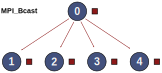
\includegraphics[width=.9\linewidth]{mpi-broadcast.pdf}}%
					\hspace{1cm}%
					\subcaptionminipage[fig:exp-gather]%
						{.35\linewidth}%
						{Example of \mpi Gather}%
						{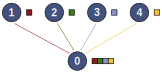
\includegraphics[width=.9\linewidth]{mpi-gather.pdf}}%

					\vspace{0.5cm}%

					\subcaptionminipage[fig:exp-allgather]%
						{.35\linewidth}%
						{Example of \mpi AllGather.}%
						{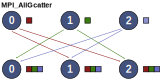
\includegraphics[width=.9\linewidth]{mpi-allgather.pdf}}%
					\hspace{1cm}%
					\subcaptionminipage[fig:exp-ping-pong]%
						{.35\linewidth}%
						{Example of Ping-Pong.}%
						{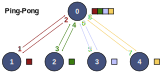
\includegraphics[width=.9\linewidth]{mpi-ping-pong.pdf}}%

					\fonte{Adapted from \citeonline{url:mpitutorial}.}%
				\end{figure}

			\subsubsection{Gather}

				\textit{Gather} is the inverse operation of a broadcast variant
				called scatter. \autoref{fig:exp-gather} illustrates the reverse
				data flow, where this routine gathers the data distributed on a
				single node~\cite{url:mpitutorial}.	Similarly to broadcast, a
				Flat Tree was implemented where all root nodes send their parts
				directly to the root node.

			\subsubsection{AllGather}

				\textit{AllGather} is a routine that does not have a root node,
				illustrated by \autoref{fig:exp-allgather}. As the name suggests,
				the routine performs several Gather operations so that all
				participating nodes end with all pieces of data gathered. Some
				possible algorithms are Ring Algorithm, Recursive Doubling, Gather
				followed by Broadcast Algorithm. The benchmark implements the
				\textit{Bruck Algorithm} where each node will send its data to a
				node with distance $i$ and receive data from a distance $-i$ until
				all nodes contain the complete data.

			\subsubsection{Ping-Pong}

				Ping-Pong is not an \mpi collective communication routine but
				represents communication from a server answering requests from
				client nodes. \autoref{fig:exp-ping-pong} illustrates
				communication by focusing on the master node, where the master
				receives and answers one request at a time.

		\subsection{Experimental Design}
		\label{subsec:experimental-design}

			The parameters that we used for each micro-benchmark are detailed
			in Table~\ref{tab:benchmarks-parameters}.
		% Portal
			The first set of experiments sought to analyze the throughput
			provided by the Portal service. All micro-benchmarks involve 1
			\iocluster and 16 \cclusters, varying the size of the buffer to
			be transmitted from 4~KB to 64~KB. Larger values were not studied
			due to limitation on physical memory size in \cclusters (\ie 2~MB).
			For instance, AllGather requires approximately a total space of
			1~MB ($17$ nodes $\times$ 64~KB).
		% Mailbox
			The second set aimed to analyze the latency of the Mailbox
			service. The micro-benchmarks executed were practically the same
			as the Portal. However, the buffer size to be transmitted became
			constant, 120~Bytes. The variable parameter of the experiments was
			the number of \cclusters involved in the routines.
			Thus, \iocluster is always the master of routines, and the number
			of \ccluster is changed between 1 and 16.

		% Quantas iterações, limitações de memória e desvio padrão
			\mppa has intrinsic characteristics that guarantee low variability
			between runs. Thus, 50 iterations of each benchmark were performed.
			For each experiment, the first ten iterations were discarded to
			eliminate undesired warm-up effects. Finally, all results discussed
			bellow preset a standard error inferior to 1\%.

			\begin{table}[!tb]
				\centering%
				\caption{Micro-benchmark parameters for experiments.}%
				\label{tab:benchmarks-parameters}%

				\begin{tabular}{l|c|c|c|l|}
					\cline{2-5}
															 & \multicolumn{2}{c|}{\textbf{\portal}}   & \multicolumn{2}{c|}{\textbf{\mailbox}} \\ \cline{2-5}
															 & \textbf{Clusters} & \textbf{Data Size}  & \textbf{Clusters} & \textbf{Data Size} \\ \hline
					\multicolumn{1}{|l|}{\textbf{Broadcast}} & 1 IO, 16 CC       & 4, 8, 16, 32, 64 KB & 1 IO, 1 to 16 CC  & 120 B              \\ \hline
					\multicolumn{1}{|l|}{\textbf{Gather}}    & 1 IO, 16 CC       & 4, 8, 16, 32, 64 KB & 1 IO, 1 to 16 CC  & 120 B              \\ \hline
					\multicolumn{1}{|l|}{\textbf{AllGather}} & 1 IO, 16 CC       & 4, 8, 16, 32, 64 KB & 1 IO, 1 to 16 CC  & 120 B              \\ \hline
					\multicolumn{1}{|l|}{\textbf{Ping-Pong}} & 1 IO, 16 CC       & 4, 8, 16, 32, 64 KB & 1 IO, 1 to 16 CC  & 120 B              \\ \hline
				\end{tabular}

				\fonte{Developed by the author.}%
			\end{table}


	\section{Result Analysis}
	\label{sec.results-analysis}

		This is a introduction of the section.

		\subsection{Portal Throughput Analysis}

			\autoref{fig:exp-portal} presents the throughput of the Portal in MB/s
			relative to the different amounts of data transmitted. Results exhibit
			three distinct behaviors in the experiments. First, the Broadcast was
			expected to have the worst transmission rate due to the use of a single
			data transmitter. Since the measurement was done on the receiver side,
			the last slave had to wait for master transmits to all other nodes,
			considerably reducing the transfer rate in the Broadcast. Second, the
			Gather and Ping-Pong routines exhibited similar results, overlapping
			each other on the chart. This similarity is because the master node
			receives multiple requests and handles them serially one by one.
			The master node dictated the data flow in both benchmarks because
			transmission is only performed when allowed by the receiver. Finally,
			the AllGather routine exhibited the best results because of the
			parallelism of communications. Also, each communication pair co-occur,
			and multiple read/write requests not happen at the same time on a node,
			softening the interruption of the master core. In the context of \oss,
			we have subsystems requiring large data transfers, such as file and
			paging systems. In this case, observing the slope of the lines,
			we can infer that the 8~KB and 16~KB sizes favor Portal throughput.
			Overall, the results were as expected, but we believe that solving
			the problem with using DMA accelerators described in
			\autoref{sec.mppa-hardware-resources} could significantly improve
			Portal performance.

			\begin{figure}[!tb]
				\centering%
				\caption{Throughput of the Portal.}%
				\label{fig:exp-portal}%
				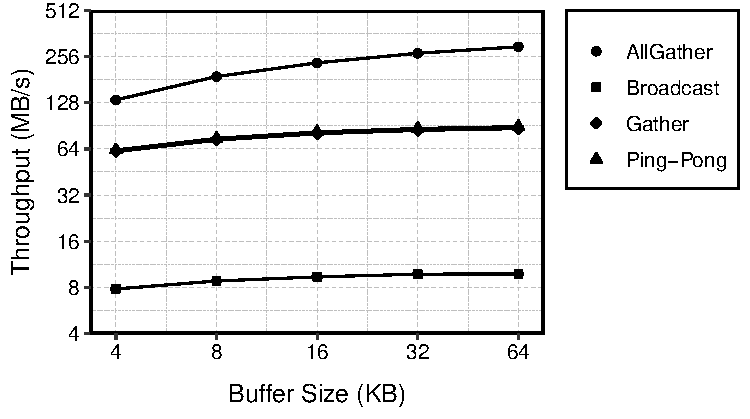
\includegraphics[width=.7\textwidth]{portal-throughput.pdf}%
				\fonte{Develop by the Author.}%
			\end{figure}

		\subsection{Mailbox Latency Analysis}

			\autoref{fig:exp-mailbox} presents the results of the experiments.
			Overall, the routines presented the expected behaviors.
			First, Gather routine, one of the essential routines, had the best
			results because receiving the messages occurs in parallel. Thus,
			the cost after the first message is the overhead of the service
			itself, not the communication. Second, AllGather routine exhibited
			similar behavior to Gather because all clusters send their messages
			before they start reading. Therefore the increase in latency is
			impacted by the transfer operation. The Broadcast routine also
			suffers from the same evil as the on Portal benchmark, where because
			exists only one node sending the messages impacts Mailbox latency.
			Finally, the linear behavior of the Ping-Pong routine is tailored
			by the overhead of sending messages to requesters. It can be noted
			that Ping-Pong has a slightly higher cost than the sum of Gather
			and Broadcast costs, where despite the benefits of receiving
			requests in parallel, the master spends most of his time handling
			requests sequentially.

			\todo[inline]{Sempre que você disser que o comportamento foi
				como o esperado, explicar antes o porque você esperava
					aquele comportamento.}

			\todo[inline]{Novamente, fazer um paralelo qualitativo dos
			resultados com o uso dessas primitivas no sistema. Ping-pong
			evidencia a latencia de comunicacao entre os subsistemas
			do Nanvix com o kernel remoto, mostrando um potencial
			para melhora com DMA pela plataforma. Broadcast, all
			gather e gather evidenciam como algoritmos
			distribuídos de concensus podem ser suportados
			de forma eficiente no multikernel.}

			\begin{figure}[!tb]
				\centering%
				\caption{Latency of the Mailbox.}%
				\label{fig:exp-mailbox}%
				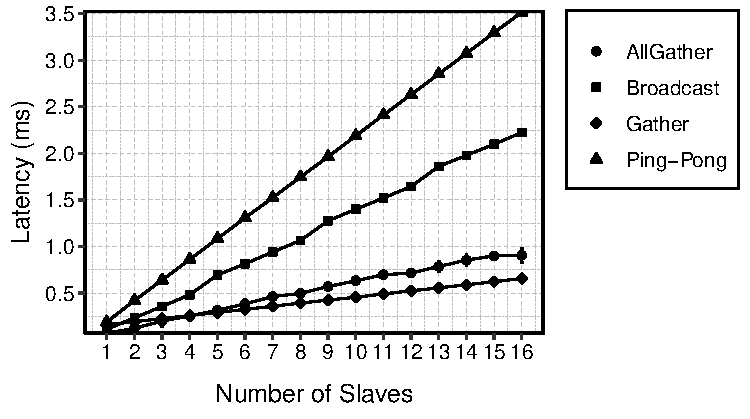
\includegraphics[width=.7\textwidth]{mailbox-latency.pdf}%
				\fonte{Develop by the Author.}%
			\end{figure}

\chapter{Schedule}
\label{ch.schedule}

This chapter presents the schedule for the next activities
planned for the development of the undergraduate dissertation.

\section{Activities}
\label{sec:gantt}

% \begin{figure}[!h]
% 	\caption{Chart Gantt of the Schedule.}

% 	\begin{center}
% 		\begin{ganttchart}[
% 			x unit=0.6cm,
% 			y unit title=0.6cm,
% 			y unit chart=0.6cm,
% 			hgrid,
% 			vgrid={{dotted, dotted, dotted, dotted, dotted, dotted}},
% 			% title label font=\3scriptsize,
% 			title/.append style={fill=gray!30},
% 			title height=1,
% 			bar/.append style={fill=gray!30,rounded corners=2pt},
% 			bar label font=\scriptsize,
% 			group label font=\scriptsize,
% 		]{7}{12}

% 		\gantttitle{\textbf{Meses}}{6} \\
% 		\gantttitle{\textbf{2019}}{6} \\
% 		\gantttitlelist{7,8,9,10,11,12}{1} \\
% 		\ganttbar{1. Writing the Implementation and Experiments.}{7}{9} \\
% 		\ganttbar{2. In-depth Writing of the Proposal.}{9}{10} \\
% 		\ganttbar{3. Presentation of the Undergraduate Dissertation.}{11}{11} \\
% 		\ganttbar{4. Review and Final Submission of the Undergraduate Dissertation.}{12}{12} \\

% 		\end{ganttchart}
% 	\end{center}

% 	\label{chart.gantt}
% \end{figure}

	ANTIGO GANTT shows the planned activities and their durations visually.
	Beginning in July 2019, the final submission is planned for December 2019.
	In detail, the activities are described below:

	\begin{itemize}
		\item \textit{Writing the Implementation and Experiments:}
			Currently, the inter-cluster communication module has the \sync abstraction
			completed and part of the \mailbox abstraction.
			Since the \portal abstraction uses the same low-level mechanisms of the others
			abstractions, its implementation will be facilitated.
			The communication services already have prototypes developed by the author
			for a symmetric \os.
			In this way, the prototypes will need to be modified to use the \hal and
			modified for a master-slave model.
			Finally, micro-benchmarks will be developed to perform an analysis of the
			performance of the implemented services.
		\item \textit{In-depth Writing of the Proposal:}
			During September and October, this activity will be committed to improving
			this draft and detailing the project decisions chose and implementations produced.
			We will also describe the experiments performed and discuss the results obtained.
		\item \textit{Presentation of the Undergraduate Dissertation:}
			November will be dedicated to the development and preparation of the presentation
			of the work and the results achieved.
			So finally, to present the dissertation to the evaluators.
		\item \textit{Review and Final Submission of the Undergraduate Dissertation:}
			Finally, December will be dedicated to the correction of the issues indicated
			by the evaluators and finalized with the final submission of the dissertation.
	\end{itemize}

 \chapter{Conclusions}
\label{ch.conclusions}

Initially, this work presented a historical context of multicore
processors to the nowadays.
By demonstrating the relationship between the growth of the number
of core and energy consumption, it was discussed how academia and
industry began to develop alternatives to alleviate the technological
barriers that have emerged.
However, even new processors that emerge and stand out because of
their performance and power consumption,
they sin in programmability and portability because of their architectural
features, such as hybrid programming model, restrictive memory subsystems,
lack of cache coherence, and heterogeneous configurations.
Part of the difficulty stems from the incompleteness of existing \oss and
runtimes in dealing with severe architectural constraints.

In this work, we present a inter-cluster communication module
designed around the main points in the development of an \os for \textit{lightweight manycores}.
As a basis, we discussed hardware and software aspects of parallel
and distributed architectures.
Different models of \os approaches have been presented that can
use the communication module.
Thus, to provide the basic functionalities for such \oss, three
communication abstractions have been proposed for \hal with the
concern of providing \qos.
Among them is the \sync abstraction to create distributed barriers.
The \mailbox abstraction provides the exchange of small messages
with flow control.
So finally, the \portal abstraction allows the exchange of
arbitrary amounts of data between two clusters.

Another contribution of this work was the communication services
for an operating system based on the microkernel approach.
These services provide for the multiplexing of the resources
exposed by \hal and the verification of the parameters required
for each abstraction.
In general, these services securely export the communication
abstractions to the user, benefiting from the non-competition
of \os internal structures because of the separation of master
and slave responsibilities.
Lastly, the proposal detailed, in general, several aspects of
the implementations.
Because the communication services depend on the \hal communication
module to be developed, the topics associated with
the module have become more detailed and better explored.
However, the next version of the undergraduate dissertation
will clearly and objectively specify both contributions of this work.


\postextual%
% Assume-se que \postextual já foi feito

\apendices

% \chapter{Exemplo de Apêndice} % e os Anexos? Eles vem antes ou depois?
% \label{ch:apendice}

% \lipsum[1]

\imprimirglossario

\imprimirindice


%%% Local Variables:
%%% mode: latex
%%% TeX-master: "main"
%%% End:


\bibliography{references}

\end{document}
